% Created 2016-06-20 一 08:43
\documentclass[xcolor=svgnames,presentation]{beamer}
\usepackage[utf8]{inputenc}
\usepackage[T1]{fontenc}
\usepackage{fixltx2e}
\usepackage{graphicx}
\usepackage{longtable}
\usepackage{float}
\usepackage{wrapfig}
\usepackage{soul}
\usepackage{textcomp}
\usepackage{marvosym}
\usepackage{wasysym}
\usepackage{latexsym}
\usepackage{amssymb}
\usepackage{hyperref}
\tolerance=1000
\usepackage{minted}
\usecolortheme[named=FireBrick]{structure}\setbeamercovered{transparent}\setbeamertemplate{caption}[numbered]\setbeamertemplate{blocks}[rounded][shadow=true] \usetheme{Darmstadt}\date{\today} \usepackage{tikz}\usepackage{xeCJK}\usepackage{amsmath}\setmainfont{Times New Roman}\setCJKmainfont[BoldFont={Adobe Heiti Std},ItalicFont={Adobe Fangsong Std}]{Adobe Heiti Std}\setCJKsansfont{Adobe Heiti Std}\setCJKmonofont{Adobe Fangsong Std}\usepackage{verbatim}\graphicspath{{figures/}} \definecolor{lstbgcolor}{rgb}{0.9,0.9,0.9} \usepackage{listings}\usepackage{minted} \usepackage{fancyvrb}\usepackage{xcolor}\lstset{escapeinside=`',frameround=ftft,language=C,breaklines=true,keywordstyle=\color{blue!70},commentstyle=\color{red!50!green!50!blue!50},frame=shadowbox,backgroundcolor=\color{yellow!20},rulesepcolor=\color{red!20!green!20!blue!20}}
\usemintedstyle{default}
\providecommand{\alert}[1]{\textbf{#1}}

\title{第12讲 防火墙与代理服务器}
\author{王晓庆}
\date{\today}
\hypersetup{
  pdfkeywords={},
  pdfsubject={},
  pdfcreator={Emacs Org-mode version 7.9.3f}}

\institute{wangxiaoqing@outlook.com}
\begin{document}

\maketitle

\begin{frame}
\frametitle{Outline}
\setcounter{tocdepth}{1}
\tableofcontents
\end{frame}
\section{概述}
\label{sec-1}
\begin{frame}
\frametitle{将内网接入Internet的主要方式}
\label{sec-1-1}
\begin{itemize}

\item 路由器
\label{sec-1-1-1}%

\item 防火墙
\label{sec-1-1-2}%

\item 代理服务器
\label{sec-1-1-3}%

\item NAT网关
\label{sec-1-1-4}%

\item VPN
\label{sec-1-1-5}%
\end{itemize} % ends low level
\begin{exampleblock}{说明}
\label{sec-1-1-6}

实际应用中,很少有使用单一方式的,往往是组合或集成上述多种方式,例如将防火墙、代理服务器和NAT进行集成。
\end{exampleblock}
\end{frame}
\begin{frame}
\frametitle{防火墙的作用}
\label{sec-1-2}
\begin{itemize}

\item 在内外网之间安装防火墙,形成一个保护层
\label{sec-1-2-1}%

\item 对进出的所有数据进行监测、分析、限制,并对用户进行认证,防止有害信息进入受保护的网络
\label{sec-1-2-2}%

\item 存在局限性,如不能防范绕过防火墙的攻击;不能防止受到病毒感染的软件或文件的传输,以及木马攻击等;难以避免来自内部的攻击
\label{sec-1-2-3}%
\end{itemize} % ends low level
\begin{columns}
\begin{column}{0.5\textwidth}
%% left
\label{sec-1-2-4}


\includegraphics[width=.9\linewidth]{img/firewall1.png}
\end{column}
\begin{column}{0.5\textwidth}
%% right
\label{sec-1-2-5}

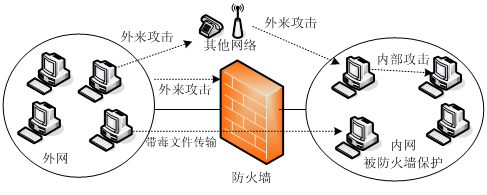
\includegraphics[width=.9\linewidth]{img/firewall2.png}
\end{column}
\end{columns}
\end{frame}
\begin{frame}
\frametitle{防火墙的类型(1)}
\label{sec-1-3}
\begin{itemize}

\item 包过滤(Packet Filtering)路由器
\label{sec-1-3-1}%
\begin{itemize}

\item 在网络层对数据包进行选择,选择的依据是设置的过滤规则,通过检查数据流中每个数据包的源地址、目的地址、所用的端口号、协议状态等因素,确定是否允许该数据包通过
\label{sec-1-3-1-1}%
\end{itemize} % ends low level

\item 应用网关
\label{sec-1-3-2}%
\begin{itemize}

\item 工作在网络体系结构的应用层,又称代理服务器,是应用级防火墙。应用网关采用代理技术提交请求和应答,不给内外网计算机直接会话机会,优点是安全,缺点是速度相对较慢。
\label{sec-1-3-2-1}%
\end{itemize} % ends low level

\item 状态检测防火墙
\label{sec-1-3-3}%
\begin{itemize}

\item 在检查数据包的基础上,也检查连接状态和应用状态信息,利用数据包之间的关联信息来避免不必要的包检查。更高级的状态检测还能基于应用状态来过滤通信
\label{sec-1-3-3-1}%
\end{itemize} % ends low level
\end{itemize} % ends low level
\end{frame}
\begin{frame}
\frametitle{防火墙的类型(2)}
\label{sec-1-4}
%% 包过滤路由器
\label{sec-1-4-1}

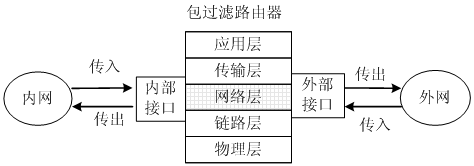
\includegraphics[width=.9\linewidth]{img/firewall3.png}
%% 应用网关
\label{sec-1-4-2}

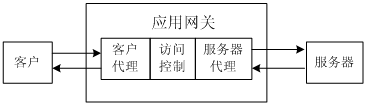
\includegraphics[width=.9\linewidth]{img/firewall4.png}
\end{frame}
\begin{frame}
\frametitle{防火墙配置方案(1)}
\label{sec-1-5}
\begin{itemize}

\item 双宿主机网关(Dual Homed Gateway)
\label{sec-1-5-1}%
\begin{itemize}

\item 用一台配有两个网络接口的双宿主机做防火墙,其中一个网络接口连接内网(被保护网络),另一个连接Internet。双宿主机又称堡垒主机,用于运行防火墙软件
\label{sec-1-5-1-1}%
\end{itemize} % ends low level
%% 示意图
\label{sec-1-5-1-2}

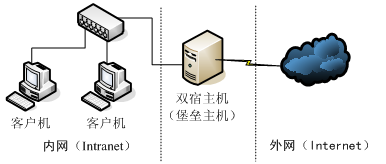
\includegraphics[width=.9\linewidth]{img/firewall5.png}
\end{itemize} % ends low level
\end{frame}
\begin{frame}
\frametitle{防火墙配置方案(2)}
\label{sec-1-6}
\begin{itemize}

\item 屏蔽主机网关(Screened Host Gateway)
\label{sec-1-6-1}%
\begin{itemize}

\item 可分为单宿型和双宿型两种类型。通常采用双宿型,堡垒主机有两块网卡,一块连接内网,一块连接包过滤路由器,双宿堡垒主机在应用层提供代理服务
\label{sec-1-6-1-1}%
\end{itemize} % ends low level
%% 示意图
\label{sec-1-6-1-2}

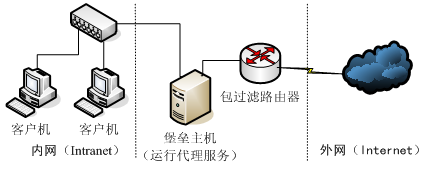
\includegraphics[width=.9\linewidth]{img/firewall6.png}
\end{itemize} % ends low level
\end{frame}
\begin{frame}
\frametitle{防火墙配置方案(3)}
\label{sec-1-7}
\begin{itemize}

\item 屏蔽子网(Screened Subnet)
\label{sec-1-7-1}%
\begin{itemize}

\item 最为复杂的防火墙体系,在内网和Internet之间建立一个被隔离的子网,该子网与内网隔离,形成一个网络防御带,在其中安装应用服务器以发布公共服务。屏蔽子网又称周边网络或DMZ。
\label{sec-1-7-1-1}%

\item 多防火墙屏蔽子网
\label{sec-1-7-1-2}%
\begin{itemize}

\item 最典型的是用两个包过滤路由器将屏蔽子网分别与内网和Internet隔开,构成一个“缓冲地带”
\label{sec-1-7-1-2-1}%
\end{itemize} % ends low level
\end{itemize} % ends low level
%% 示意图
\label{sec-1-7-1-3}

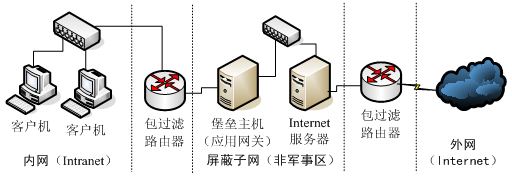
\includegraphics[width=.9\linewidth]{img/firewall7.png}
\end{itemize} % ends low level
\end{frame}
\begin{frame}
\frametitle{防火墙配置方案(4)}
\label{sec-1-8}
\begin{itemize}

\item 三宿主机屏蔽子网
\label{sec-1-8-1}%
\begin{itemize}

\item 一台防火墙主机共有3个网络接口,分别连接到内部专用网、屏蔽网络和外网(Internet)
\label{sec-1-8-1-1}%
\end{itemize} % ends low level
%% 示意图
\label{sec-1-8-1-2}

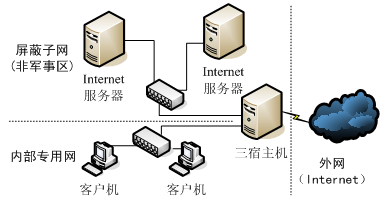
\includegraphics[width=.9\linewidth]{img/firewall8.png}
\end{itemize} % ends low level
\end{frame}
\begin{frame}
\frametitle{Linux防火墙解决方案}
\label{sec-1-9}
\begin{itemize}

\item Linux提供优秀的防火墙软件Netfilter/iptables,可以在一台低配置的计算机上运行,以替代昂贵的硬件防火墙产品
\label{sec-1-9-1}%

\item 就功能特性来说,可以将防火墙分为以下3种类型:
\label{sec-1-9-2}%
\begin{enumerate}
\item NAT:让内网通过一个或多个公网IP地址访问公网,作为一种防火墙技术,将内网IP地址隐藏起来使公网用户无法直接访问内网。
\item 包过滤:依据过滤规则读取和处理网关的所有数据包,允许或阻止数据包通过网关,是一种最基本的防火墙技术。
\item 代理服务器:代表内网主机与外部主机通信,通常是应用级网关。作为防火墙技术,隔离内外网,并提供访问控制和网络监控功能。
\end{enumerate}
\end{itemize} % ends low level
\end{frame}
\begin{frame}
\frametitle{Linux的NAT技术}
\label{sec-1-10}
\begin{itemize}

\item Linux的Netfilter/iptables支持源NAT和目的NAT。
\label{sec-1-10-1}%

\item NAT对数据包的源IP地址、目的IP地址、源端口、目的端口进行改写,据此将NAT分为以下两种类型:
\label{sec-1-10-2}%
\begin{enumerate}
\item 源NAT(SNAT)
\end{enumerate}
改变数据包的源地址。网络连接共享属于源NAT,IP伪装(IP Masquerade)是源NAT的一种特殊形式。
\begin{enumerate}
\item 目的NAT(DNAT)
\end{enumerate}
改变数据包的目的地址,它与源NAT相反。例如,端口转发、负载均衡和透明代理就是属于目的NAT。
\end{itemize} % ends low level
\end{frame}
\begin{frame}
\frametitle{代理服务器技术(1)}
\label{sec-1-11}
\begin{itemize}

\item 代理服务器工作原理
\label{sec-1-11-1}%
\begin{itemize}

\item 应用层代理是最典型的代理方式,狭义的代理服务往往指这种方式
\label{sec-1-11-1-1}%

\item 在客户端和服务器之间建立连接并转发数据
\label{sec-1-11-1-2}%

\item 工作在应用层,多数代理服务器只支持部分应用程序,一般支持HTTP代理
\label{sec-1-11-1-3}%

\item 复杂的应用层代理还能够缓存、过滤和优化数据
\label{sec-1-11-1-4}%

\item 代理服务器至少有两个网络接口,一个连接内网,另一个连接Internet
\label{sec-1-11-1-5}%
\end{itemize} % ends low level
\end{itemize} % ends low level
%% 示意图
\label{sec-1-11-2}

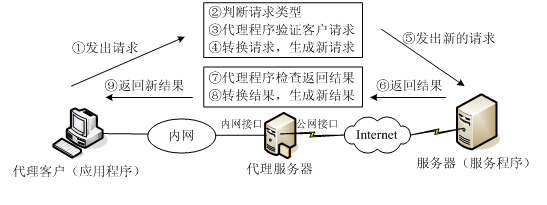
\includegraphics[width=.9\linewidth]{img/agent1.png}
\end{frame}
\begin{frame}
\frametitle{代理服务器技术(2)}
\label{sec-1-12}
\begin{itemize}

\item 反向代理技术\\
\label{sec-1-12-1}%
代理服务器也可为外网用户访问内网提供代理服务,通常将这种代理服务称为反向代理或逆向代理
\begin{itemize}

\item 通常只用来发布内网Web服务器
\label{sec-1-12-1-1}%

\item 不仅充当防火墙以防止外网用户直接与Web服务器通信,还可充当Web缓冲服务器,以降低实际Web服务器负载,提高访问速度
\label{sec-1-12-1-2}%

\item 可对用户身份进行认证,对访问内容进行过滤
\label{sec-1-12-1-3}%

\item 常用于网络负载均衡和故障热处理,对性能要求很高。
\label{sec-1-12-1-4}%
\end{itemize} % ends low level
\end{itemize} % ends low level
%% 示意图
\label{sec-1-12-2}

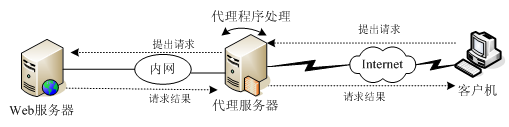
\includegraphics[width=.9\linewidth]{img/agent2.png}
\end{frame}
\begin{frame}
\frametitle{代理服务器技术(3)}
\label{sec-1-13}
\begin{itemize}

\item 缓存(代理缓存服务器)
\label{sec-1-13-1}%
\begin{itemize}

\item 缓存由一个或多个分区组成,此处分区是指磁盘上用作缓存的存储区域
\label{sec-1-13-1-1}%

\item 当使用代理缓存时,用户的Web请求被发送到代理服务器
\label{sec-1-13-1-2}%

\item 代理服务器首先请求缓存中的Web信息,如果缓存中没有,就向源Web服务器请求信息并将其存入缓存中,然后再发送信息给请求的用户
\label{sec-1-13-1-3}%
\end{itemize} % ends low level

\item 缓存方案主要有3种类型
\label{sec-1-13-2}%
\begin{enumerate}
\item 标准代理缓存(正向代理)
\item HTTP(Web)加速器(即反向代理)
\item ICP(Internet缓存协议)多层缓存
\end{enumerate}
\end{itemize} % ends low level
\end{frame}
\begin{frame}
\frametitle{代理服务器技术(4)}
\label{sec-1-14}
\begin{itemize}

\item 标准代理缓存\\
\label{sec-1-14-1}%
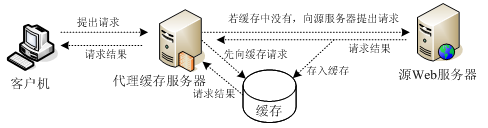
\includegraphics[width=.9\linewidth]{img/agent3.png}

\item ICP多层缓存\\
\label{sec-1-14-2}%
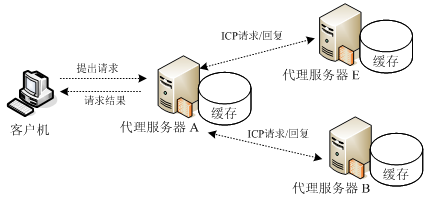
\includegraphics[width=.9\linewidth]{img/agent4.png}
\end{itemize} % ends low level
\end{frame}
\section{Netfilter/iptables基础}
\label{sec-2}
\begin{frame}
\frametitle{Netfilter架构(1)}
\label{sec-2-1}
\begin{itemize}

\item 概述
\label{sec-2-1-1}%
\begin{itemize}

\item Netfilter位于网络层与防火墙内核之间,是Linux内核中的一个通用架构,定义了包过滤子系统功能的实现。
\label{sec-2-1-1-1}%

\item iptables使用Netfilter架构在Linux内核中管理包过滤
\label{sec-2-1-1-2}%

\item Netfilter提供3个表(tables),每个表由若干个链(chains)组成,而每条链可以由若干条规则(rules)组成
\label{sec-2-1-1-3}%

\item 可以将Netfilter看成是表的容器,将表看成是链的容器,将链看成是规则的容器
\label{sec-2-1-1-4}%

\item 表是所有规则的总和,链是在某一检查点上的规则的集合。
\label{sec-2-1-1-5}%
\end{itemize} % ends low level
\end{itemize} % ends low level
%% 示意图
\label{sec-2-1-2}

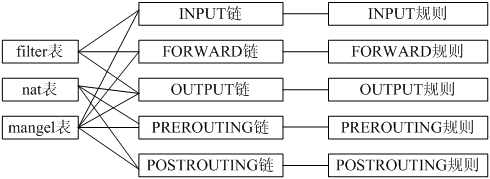
\includegraphics[width=.9\linewidth]{img/iptables1.png}
\end{frame}
\begin{frame}
\frametitle{Netfilter架构(2)}
\label{sec-2-2}
\begin{itemize}

\item 表
\label{sec-2-2-1}%
\begin{itemize}

\item filter(过滤网络数据包)
\label{sec-2-2-1-1}%

\item nat(修改数据包来创建新的连接,实现网络地址转换)
\label{sec-2-2-1-2}%

\item mangle(处理特定的数据包)
\label{sec-2-2-1-3}%
\end{itemize} % ends low level
\end{itemize} % ends low level
\end{frame}
\begin{frame}
\frametitle{Netfilter架构(3)}
\label{sec-2-3}
\begin{itemize}

\item 链
\label{sec-2-3-1}%
\begin{itemize}

\item filter表内置链
\label{sec-2-3-1-1}%
\begin{itemize}

\item INPUT(处理目标地址是本机的网络数据包,即检测过滤传入数据包)
\label{sec-2-3-1-1-1}%

\item FORWARD(处理经本机转发的数据包,即检测过滤路由数据包)
\label{sec-2-3-1-1-2}%

\item OUTPUT(处理由本地产生要发送的网络数据包,即检测过滤传出数据包)
\label{sec-2-3-1-1-3}%
\end{itemize} % ends low level

\item nat表内置链
\label{sec-2-3-1-2}%
\begin{itemize}

\item PREROUTING(包含路由前的规则,转换需要转发数据包的目的地址)
\label{sec-2-3-1-2-1}%

\item POSTROUTTNG(包含路由后的规则,转换需要转发数据包的源地址)
\label{sec-2-3-1-2-2}%

\item OUTPUT(转换本地数据包的目的地址)
\label{sec-2-3-1-2-3}%
\end{itemize} % ends low level

\item mangle表内置链
\label{sec-2-3-1-3}%
\begin{itemize}

\item INPUT、OUTPUT、FORWARD、PRFROUTTNG和POSTROUTTNG
\label{sec-2-3-1-3-1}%
\end{itemize} % ends low level
\end{itemize} % ends low level
\end{itemize} % ends low level
\end{frame}
\begin{frame}
\frametitle{Netfilter架构(4)}
\label{sec-2-4}
\begin{itemize}

\item 规则
\label{sec-2-4-1}%
\begin{itemize}

\item 每一条链中可以有一条或多条规则
\label{sec-2-4-1-1}%

\item 每条规则定义所要检查的数据包的特征或条件,如源地址、目的地址、传输协议等,以及处理匹配条件的包的方法,如允许、拒绝等
\label{sec-2-4-1-2}%

\item 当一个数据包到达一个链时,iptables从链中第1条规则开始检查,判断该数据包是否满足规则所定义的条件,如果满足就按照所定义的方法处理该数据包;否则继续检查下一条规则,如果不符合链中任何规则,iptables根据该链预定义的默认策略来处理数据包
\label{sec-2-4-1-3}%
\end{itemize} % ends low level
\end{itemize} % ends low level
\end{frame}
\begin{frame}
\frametitle{Netfilter架构(5)}
\label{sec-2-5}
\begin{itemize}

\item 包处理流程
\label{sec-2-5-1}%
\begin{itemize}

\item 数据包到达Linux网络接口,根据定义的规则进行处理
\label{sec-2-5-1-1}%

\item 涉及Netfilter的3个表(filter、nat和mangle),每个表又有不同的链
\label{sec-2-5-1-2}%

\item filter表用于实现防火墙功能,内置的3个链INPUT、FORWAR和OUTPUT,分别对包的传入、转发和传出进行过滤处理
\label{sec-2-5-1-3}%

\item nat表用于实现地址转换和端口转发功能,内置的3个链PREROUTING、POSTROUTING和OUTPUT,分别对转发数据包目的地址、转发数据包源地址和本地数据包目的地址进行转换。
\label{sec-2-5-1-4}%

\item mangle表则是一个自定义表,用于各种自定义操作,而且mangle表中的链在Netfilter包处理流程中处于优先的位置。实际应用中很少用到mangle表。
\label{sec-2-5-1-5}%
\end{itemize} % ends low level
\end{itemize} % ends low level
\end{frame}
\begin{frame}
\frametitle{Netfilter架构(6)}
\label{sec-2-6}
%% Netfilter包处理流程
\label{sec-2-6-1}

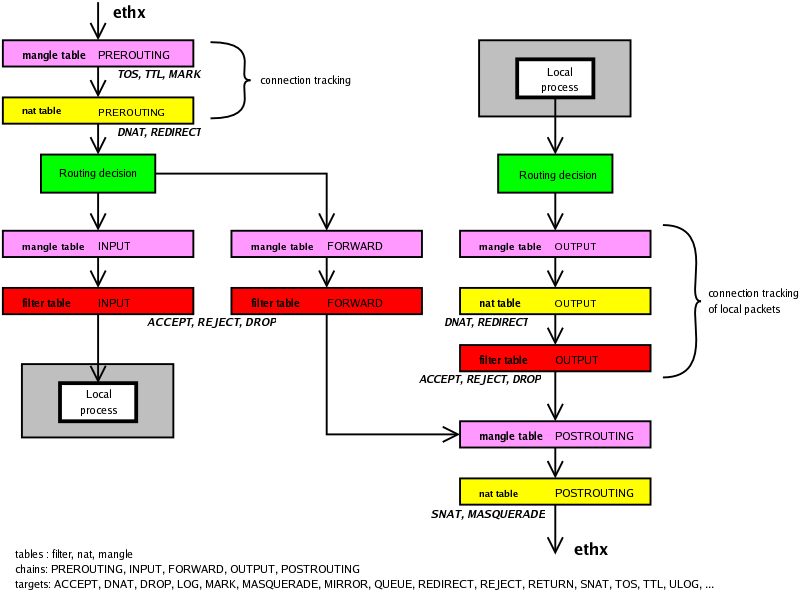
\includegraphics[width=.9\linewidth]{img/iptables.png}
\end{frame}
\begin{frame}
\frametitle{包过滤机制(1)}
\label{sec-2-7}
\begin{itemize}

\item filter表用于实现包的过滤处理,内置3个链:
\label{sec-2-7-1}%
\begin{itemize}

\item INPUT链过滤从内网或外网发往防火墙本身的数据包
\label{sec-2-7-1-1}%

\item OUTPUT链过滤从防火墙本身发往内网或外网的数据包
\label{sec-2-7-1-2}%

\item FORWARD链过滤内外网之间通过防火墙转发的数据包
\label{sec-2-7-1-3}%

\item 除了3个内置链之外,管理员可根据需要添加自定义的链
\label{sec-2-7-1-4}%
\end{itemize} % ends low level

\item 当数据包到达防火墙时,Linux内核首先根据路由表决定数据包的目标,若数据包的目的地址是本机,则将数据包送往INPUT链进行规则检查;若目的地址不是本机,则检查内核是否允许转发,如果允许,则将数据包送往FORWARD链进行规则检查,如果不允许转发,则丢弃该数据包。对于防火墙主机本地进程产生并准备发出的数据包,则交由OUTPUT链进行规则检查。
\label{sec-2-7-2}%
\end{itemize} % ends low level
\end{frame}
\begin{frame}
\frametitle{包过滤机制(2)}
\label{sec-2-8}
%% 包过滤机制
\label{sec-2-8-1}

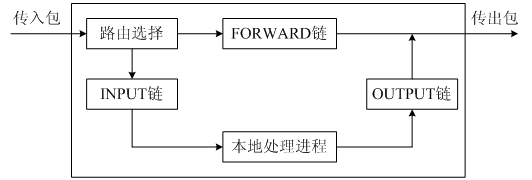
\includegraphics[width=.9\linewidth]{img/iptables3.png}
\end{frame}
\begin{frame}
\frametitle{包过滤机制(3)}
\label{sec-2-9}
\begin{itemize}

\item 包通信方向
\label{sec-2-9-1}%
\begin{itemize}

\item 应正确理解每个接口上数据通信的方向
\label{sec-2-9-1-1}%

\item 同一数据包通过不同的网络接口,通信方向不同
\label{sec-2-9-1-2}%

\item 从内网到外网的通信,在内网接口上为传入通信,在外网接口上为传出通信
\label{sec-2-9-1-3}%

\item 从外网到内网的通信,在外网接口上为传入通信,在内网接口上为传出通信
\label{sec-2-9-1-4}%
\end{itemize} % ends low level
\end{itemize} % ends low level
%% 包通信方向
\label{sec-2-9-2}

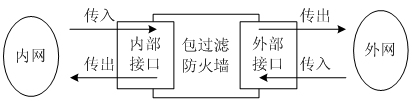
\includegraphics[width=.9\linewidth]{img/iptables4.png}
\end{frame}
\begin{frame}
\frametitle{网络地址转换机制(1)}
\label{sec-2-10}
\begin{itemize}

\item 网络地址转换类型
\label{sec-2-10-1}%
\begin{itemize}

\item 数据包的源地址(或端口)或目的地址(或端口)修改需要通过nat表来实现
\label{sec-2-10-1-1}%

\item 对源地址或源端口进行替换修改,称为SNAT(源NAT)
\label{sec-2-10-1-2}%

\item 对目的地址或端口进行替换修改,称为DNAT(目的NAT)
\label{sec-2-10-1-3}%
\end{itemize} % ends low level
\end{itemize} % ends low level
\end{frame}
\begin{frame}
\frametitle{网络地址转换机制(2)}
\label{sec-2-11}
\begin{itemize}

\item nat链
\label{sec-2-11-1}%
\begin{itemize}

\item INPUT链过滤从内网或外网发往防火墙本身的数据包
\label{sec-2-11-1-1}%

\item OUTPUT链过滤从防火墙本身发往内网或外网的数据包
\label{sec-2-11-1-2}%

\item FORWARD链过滤内外网之间通过防火墙转发的数据包
\label{sec-2-11-1-3}%
\end{itemize} % ends low level

\item 网络地址转换过程
\label{sec-2-11-2}%
\begin{itemize}

\item 当数据包到达防火墙时,在还没有交给路由选择之前由PREROUTING链进行检查处理,该链可以对需要转发的数据包的目的地址和端口进行转换修改(DNAT),从而实现端口或主机重定向
\label{sec-2-11-2-1}%

\item 经过路由选择之后,所有要传出的包在POSTROUTING链中进行检查处理,该链可以对包的源地址或端口进行转换修改(SNAT)。
\label{sec-2-11-2-2}%

\item 本地进程产生并准备传出的包则由OUTPUT链进行检查处理,该链也可进行DNAT操作。
\label{sec-2-11-2-3}%
\end{itemize} % ends low level
\end{itemize} % ends low level
\end{frame}
\begin{frame}
\frametitle{网络地址转换机制(3)}
\label{sec-2-12}
%% 网络地址转换机制
\label{sec-2-12-1}

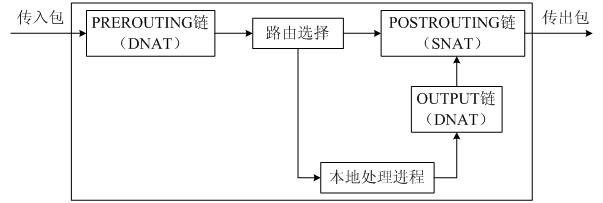
\includegraphics[width=.9\linewidth]{img/iptables5.png}
\end{frame}
\begin{frame}[fragile]
\frametitle{iptables命令组成}
\label{sec-2-13}
\begin{itemize}

\item iptables命令格式\\
\label{sec-2-13-1}%
\begin{minted}[]{bash}
iptables [-t table] cmd chain [options]
\end{minted}

\item 说明
\label{sec-2-13-2}%
\begin{itemize}

\item table:指定这个规则所应用的规则表(filter, nat, mangle),如果没有使用这个选项,默认指定filter表
\label{sec-2-13-2-1}%

\item cmd:指定要执行的动作,如添加或删除一条规则
\label{sec-2-13-2-2}%

\item chain:指定编辑、创建或删除的链
\label{sec-2-13-2-3}%

\item options:选项,如匹配规则和/或动作
\label{sec-2-13-2-4}%
\end{itemize} % ends low level
\end{itemize} % ends low level
\end{frame}
\begin{frame}[fragile]
\frametitle{iptables命令(1)}
\label{sec-2-14}
\begin{exampleblock}{-A(--append)}
\label{sec-2-14-1}


\begin{minted}[]{bash}
iptables -A INPUT -j ACCEPT
#向filter表的INPUT链追加一条规则:
#接受所有目标地址为本机的数据包
#新增加的规则将会成为规则链中的最后一条规则
\end{minted}
\end{exampleblock}
\begin{block}{-D(--delete)}
\label{sec-2-14-2}


\begin{minted}[]{bash}
iptables -D INPUT -p tcp --dport 80 -j DROP
#从filter表中删除规则:
#拒绝协议为tcp,目标地址为本机80端口的数据包
#也可以通过指定规则编号加以删除,如:
iptables -D INPUT 1 #删除INPUT链中编号为1的规则
\end{minted}
\end{block}
\end{frame}
\begin{frame}[fragile]
\frametitle{iptables命令(2)}
\label{sec-2-15}
\begin{exampleblock}{-I(--insert)}
\label{sec-2-15-1}


\begin{minted}[]{bash}
iptables -I INPUT 1 -p tcp --dport 80 -j ACCEPT
#在filter表的INPUT链中位置1处插入一条规则:
#允许协议为tcp,目标地址为本机80端口的数据包
#原来在位置1及其后的规则依次向后移动
\end{minted}
\end{exampleblock}
\begin{block}{--L(--list)}
\label{sec-2-15-2}


\begin{minted}[]{bash}
iptables -L INPUT
#列出filter表的INPUT链中的所有规则
iptables -L #列出filter表的所有规则
iptables -t nat -L #列出nat表的所有规则
\end{minted}
\end{block}
\end{frame}
\begin{frame}[fragile]
\frametitle{iptables命令(3)}
\label{sec-2-16}
\begin{exampleblock}{-F(--flush)}
\label{sec-2-16-1}


\begin{minted}[]{bash}
iptables -F INPUT
#清空filter表的INPUT链中的所有规则
iptables -t nat -F
#清空nat表的所有规则
\end{minted}
\end{exampleblock}
\begin{block}{-Z(--zero)}
\label{sec-2-16-2}


\begin{minted}[]{bash}
iptables -Z INPUT
#将filter表的INPUT链的计数器清零
iptables -Z
#将filter表的所有链的计数器清零
\end{minted}
\end{block}
\end{frame}
\begin{frame}[fragile]
\frametitle{iptables命令(4)}
\label{sec-2-17}
\begin{exampleblock}{-R(--replace)}
\label{sec-2-17-1}


\begin{minted}[]{bash}
iptables -R INPUT 1 -p tcp --dport 80 -j DROP
#替换filter表的INPUT链的规则1:
#丢弃目标地址为本机tcp协议80端口的数据包
\end{minted}
\end{exampleblock}
\begin{block}{-P(--policy)}
\label{sec-2-17-2}


\begin{minted}[]{bash}
iptables -P INPUT DROP
#设置filter表的INPUT链的默认处理策略为DROP
#当数据包经过INPUT链且没有匹配任何规则时将被丢弃
#只有内置链才能定义默认处理策略
\end{minted}
\end{block}
\end{frame}
\begin{frame}[fragile]
\frametitle{iptables命令(5)}
\label{sec-2-18}
\begin{exampleblock}{-N(--new-chain)}
\label{sec-2-18-1}


\begin{minted}[]{bash}
iptables -N MYCHAIN
#在filter表中定义一条名为MYCHAIN的新链
#定义了新链后,可以在新链中添加规则
\end{minted}
\end{exampleblock}
\begin{block}{-X(--delete-chain)}
\label{sec-2-18-2}


\begin{minted}[]{bash}
iptables -X MYCHAIN
#删除filter表中名为MYCHAIN的链
#只能删除用户自定义的链,不能删除内置链
#被删除的自定义链必须没有被引用
\end{minted}
\end{block}
\begin{exampleblock}{-E(--rename-chain)}
\label{sec-2-18-3}


\begin{minted}[]{bash}
iptables -E MYCHAIN MYNEWCHAIN
#将用户自定义的链MYCHAIN重命名为MYNEWCHAIN
\end{minted}
\end{exampleblock}
\end{frame}
\begin{frame}[fragile]
\frametitle{iptables匹配参数(1)}
\label{sec-2-19}
\begin{exampleblock}{-p(--protocol)}
\label{sec-2-19-1}


\begin{minted}[]{bash}
iptables -A INPUT -p tcp -j ACCEPT
#-p可以匹配协议类型tcp,udp,icmp或all
#-p ! tcp表示匹配tcp之外的其他协议
\end{minted}
\end{exampleblock}
\begin{block}{-s(--source)}
\label{sec-2-19-2}


\begin{minted}[]{bash}
iptables -A INPUT -s 192.168.1.1 -j ACCEPT
#允许源地址为192.168.1.1且目的地址为本机的数据包
#-s 192.168.1.0/24匹配一个网段的源地址
#-s ! 192.168.2.0/24排除一个网段的源地址
\end{minted}
\end{block}
\end{frame}
\begin{frame}[fragile]
\frametitle{iptables参数(2)}
\label{sec-2-20}
\begin{exampleblock}{-d(--destination)}
\label{sec-2-20-1}


\begin{minted}[]{bash}
iptables -A OUTPUT -d 192.168.1.1 -j ACCEPT
#允许源地址为本机且目的地址为192.168.1.1的数据包
\end{minted}
\end{exampleblock}
\begin{block}{-j(--jump)}
\label{sec-2-20-2}


\begin{minted}[]{bash}
#定义规则的目标,即对匹配该规则的数据包所做的操作。
#目标可以是用户自定义链
#目标也可以是一个内置目标(ACCEPT,DROP等)或扩展
\end{minted}
\end{block}
\begin{exampleblock}{-g(--goto)}
\label{sec-2-20-3}


\begin{minted}[]{bash}
#设置数据包继续到用户自定义链进行处理
\end{minted}
\end{exampleblock}
\end{frame}
\begin{frame}[fragile]
\frametitle{iptables参数(3)}
\label{sec-2-21}
\begin{exampleblock}{-i(--in-interface)}
\label{sec-2-21-1}


\begin{minted}[]{bash}
iptables -A INPUT -i eth0 -j ACCEPT
#允许从eth0接口进入且目的地值为本机的数据包
\end{minted}
\end{exampleblock}
\begin{block}{-o(--out-interface)}
\label{sec-2-21-2}


\begin{minted}[]{bash}
iptables -A FORWARD -o eth1 -j ACCEPT
#允许源地址和目的地址都不是本机从eth1接口转发出去
\end{minted}
\end{block}
\end{frame}
\begin{frame}[fragile]
\frametitle{iptables参数(4)}
\label{sec-2-22}
\begin{exampleblock}{-f(--fragment)}
\label{sec-2-22-1}


\begin{minted}[]{bash}
#设置只对分段(分片)的数据包应用当前规则
\end{minted}
\end{exampleblock}
\begin{block}{-c(--set-counters) PKTS BYTES}
\label{sec-2-22-2}


\begin{minted}[]{bash}
#为指定规则重设(初始化)计数器,可指定重设的包计数器或字节计数器
\end{minted}
\end{block}
\end{frame}
\begin{frame}[fragile]
\frametitle{iptables匹配扩展(1)}
\label{sec-2-23}
\begin{itemize}

\item 不同的网络协议提供不同的匹配扩展,前提是该协议必须现在iptables指令中指定。
\label{sec-2-23-1}%

\item -p tcp的匹配扩展
\label{sec-2-23-2}%
\begin{exampleblock}{--sport(--source-port)}
\label{sec-2-23-2-1}


\begin{minted}[]{bash}
iptables -A INPUT -p tcp --sport 1:1024 -j ACCEPT
#允许源端口号为1-1024且目的地址为本机的tcp包
\end{minted}
\end{exampleblock}
\begin{block}{--dport(--destination-port)}
\label{sec-2-23-2-2}


\begin{minted}[]{bash}
iptables -A OUTPUT -p tcp --dport 80 -j ACCEPT
#允许从本机发出的目标端口号为80的tcp包
\end{minted}
\end{block}
\begin{exampleblock}{--syn}
\label{sec-2-23-2-3}


\begin{minted}[]{bash}
--syn 匹配syn包,! --syn 匹配非syn包
\end{minted}
\end{exampleblock}
\end{itemize} % ends low level
\end{frame}
\begin{frame}[fragile]
\frametitle{iptables匹配扩展(2)}
\label{sec-2-24}
\begin{itemize}

\item -p tcp的匹配扩展(续)
\label{sec-2-24-1}%
\begin{exampleblock}{--tcp-flags}
\label{sec-2-24-1-1}


\begin{minted}[]{bash}
iptables -A FORWARD -p tcp --tcp-flags SYN,ACK,FIN,RST SYN
#检查数据包的SYN,ACK,FIN,RST位
#仅匹配设置了SYN位,而未设置ACK,FIN,RST位的数据包
\end{minted}
\end{exampleblock}
\begin{block}{--tcp-options}
\label{sec-2-24-1-2}


\begin{minted}[]{bash}
iptables -A FORWARD -p tcp --tcp-options 6
#检查tcp选项类型,匹配选项类型为6的数据包
#选项类型值可参考
http://www.iana.org/assignments/
tcp-parameters/tcp-parameters.xhtml
\end{minted}
\end{block}
\end{itemize} % ends low level
\end{frame}
\begin{frame}[fragile]
\frametitle{iptables匹配扩展(2)}
\label{sec-2-25}
\begin{itemize}

\item -p udp的匹配扩展
\label{sec-2-25-1}%
\begin{itemize}

\item --sport
\label{sec-2-25-1-1}%

\item --dport
\label{sec-2-25-1-2}%
\end{itemize} % ends low level

\item -p icmp的匹配扩展
\label{sec-2-25-2}%
\begin{exampleblock}{--icmp-type}
\label{sec-2-25-2-1}


\begin{minted}[]{bash}
iptables -A INPUT -p icmp --icmp-type 8 -j ACCEPT
#允许目标地址为本机且类型值为8(echo request)的icmp包
#可以写类型值或类型名
iptables -p icmp -h #可查看icmp类型列表
\end{minted}
\end{exampleblock}
\end{itemize} % ends low level
\end{frame}
\begin{frame}[fragile]
\frametitle{iptables匹配扩展(3)}
\label{sec-2-26}
\begin{exampleblock}{-m limit的匹配扩展}
\label{sec-2-26-1}


\begin{minted}[]{bash}
iptables -A INPUT -m limit --limit 100/s \
--limit-burst 120 -j ACCEPT
#突发收到120个数据包后立即触发
#每秒仅允许通过100个数据包的限制
#--limit的时间单位可以是s(秒),m(分),h(时),d(日)
\end{minted}
\end{exampleblock}
\begin{block}{-m mac的匹配扩展}
\label{sec-2-26-2}


\begin{minted}[]{bash}
iptables -A FORWARD -m mac \
--mac-source 00:50:0C:34:9A:D3 -j DROP
#丢弃来自指定MAC地址发出的数据包
#注意:一个数据包经过路由器转发后,
#     其源MAC地址将变成路由器接口的MAC地址!
\end{minted}
\end{block}
\end{frame}
\begin{frame}
\frametitle{iptables目标选项(1)}
\label{sec-2-27}
\begin{itemize}

\item 当一个数据包与一个特定的规则相匹配时,这条规则可以将这个数据包重新定向到不同的目标中,由这些目标来决定对这个数据包如何处理。目标选项通过-j参数指定,可分为3种类型
\label{sec-2-27-1}%

\item 标准的目标选项
\label{sec-2-27-2}%
\begin{itemize}

\item ACCEP:允许数据包通过并发送到它的目的地或其他链。
\label{sec-2-27-2-1}%

\item DROP:丢弃数据包,不给发送者任何反馈信息。
\label{sec-2-27-2-2}%

\item QUEUE:将数据包放置在一个用户空间应用程序的队列中等待被处理。
\label{sec-2-27-2-3}%

\item RETURN:停止遍历当前链中的规则,恢复到先前链的下一条规则。
\label{sec-2-27-2-4}%
\end{itemize} % ends low level
\end{itemize} % ends low level
\end{frame}
\begin{frame}
\frametitle{iptables目标选项(2)}
\label{sec-2-28}
\begin{itemize}

\item 扩展的目标模块
\label{sec-2-28-1}%
\begin{itemize}

\item LOG:在日志中记录所有匹配这条规则的数据包
\label{sec-2-28-1-1}%

\item REJECT:丢弃数据包,并向远程系统发回一个错误通知
\label{sec-2-28-1-2}%

\item MASQUERADE:将数据包来源IP转换为输出数据包的接口的IP以实现IP伪装。
\label{sec-2-28-1-3}%

\item SNAT:将数据包来源IP和端口转换为某指定的IP和端口。
\label{sec-2-28-1-4}%

\item DNAT:将数据包目的IP和端口转换为某指定的IP和端口。
\label{sec-2-28-1-5}%

\item REDIRECT:将数据包重新转向到本机或另一台主机的某个端口,通常用此功能实现透明代理或对外开放内网,它相当于DNAT的一个特例。
\label{sec-2-28-1-6}%
\end{itemize} % ends low level

\item 自定义链
\label{sec-2-28-2}%
\begin{itemize}

\item 规则的目标也可以是一个自定义链的名称,该链应事先建立好,并在链中设置好相应的规则。
\label{sec-2-28-2-1}%
\end{itemize} % ends low level
\end{itemize} % ends low level
\end{frame}
\begin{frame}
\frametitle{iptables命令练习(1)}
\label{sec-2-29}
%% 现有网络拓扑结构如下图:
\label{sec-2-29-1}

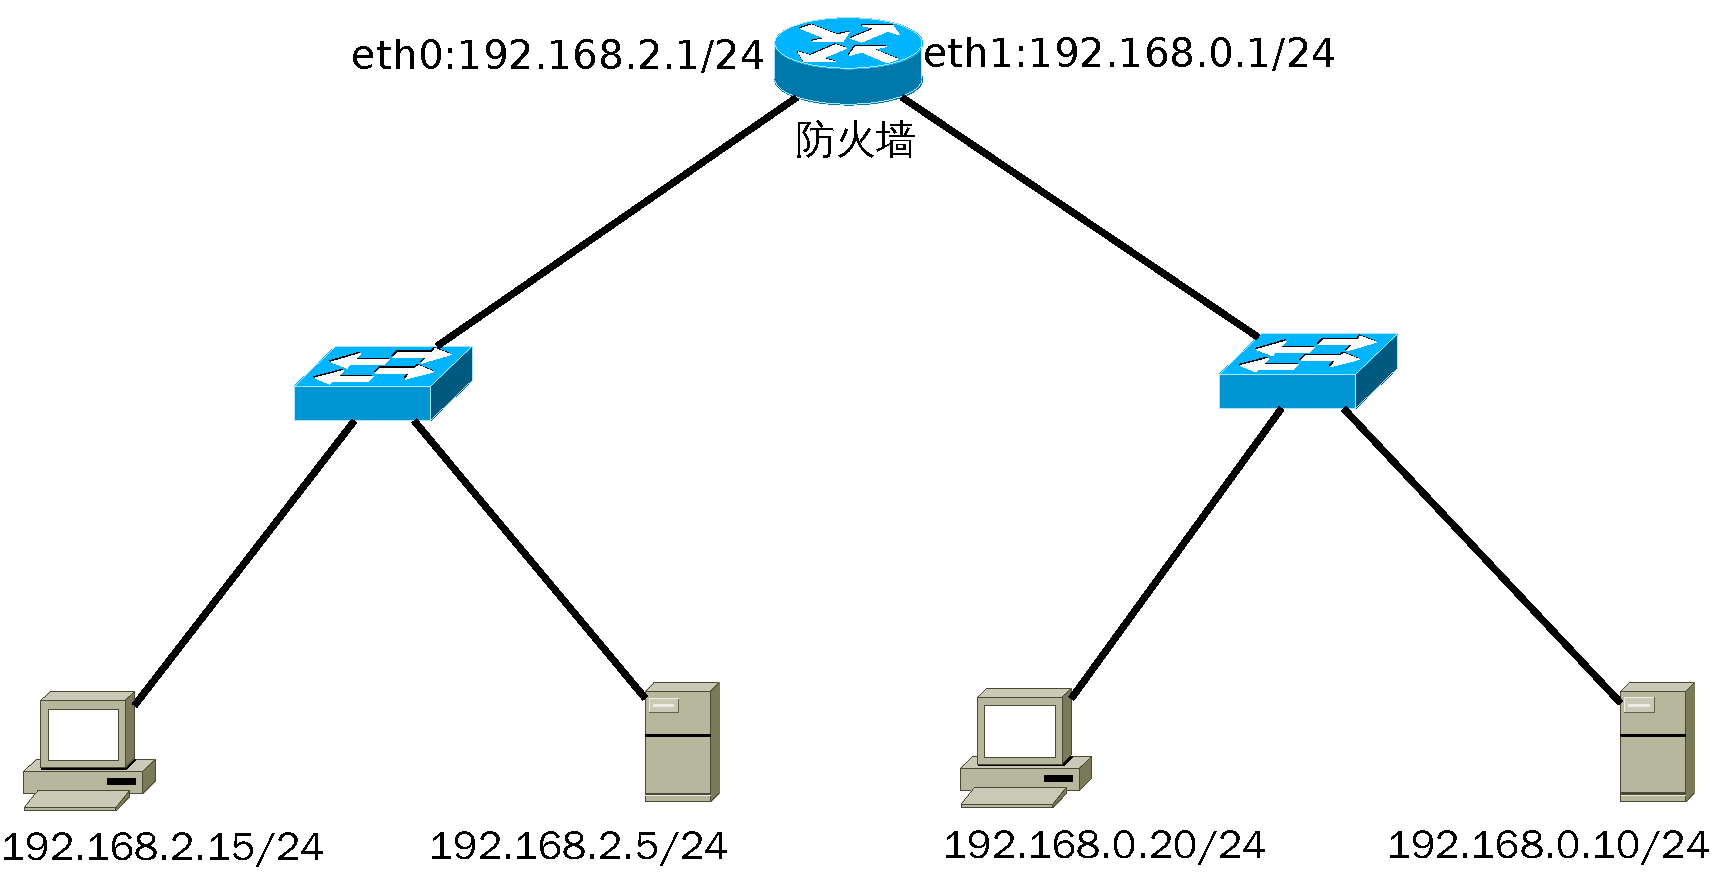
\includegraphics[width=.9\linewidth]{img/iptables-test.pdf}
\begin{itemize}

\item 1. 如果在防火墙上执行iptables -A INPUT -p icmp -j DROP,请问192.168.2.15及192.168.0.20谁可以ping到防火墙?
\label{sec-2-29-2}%
\end{itemize} % ends low level
\end{frame}
\begin{frame}
\frametitle{iptables命令练习(2)}
\label{sec-2-30}
%% 图
\label{sec-2-30-1}

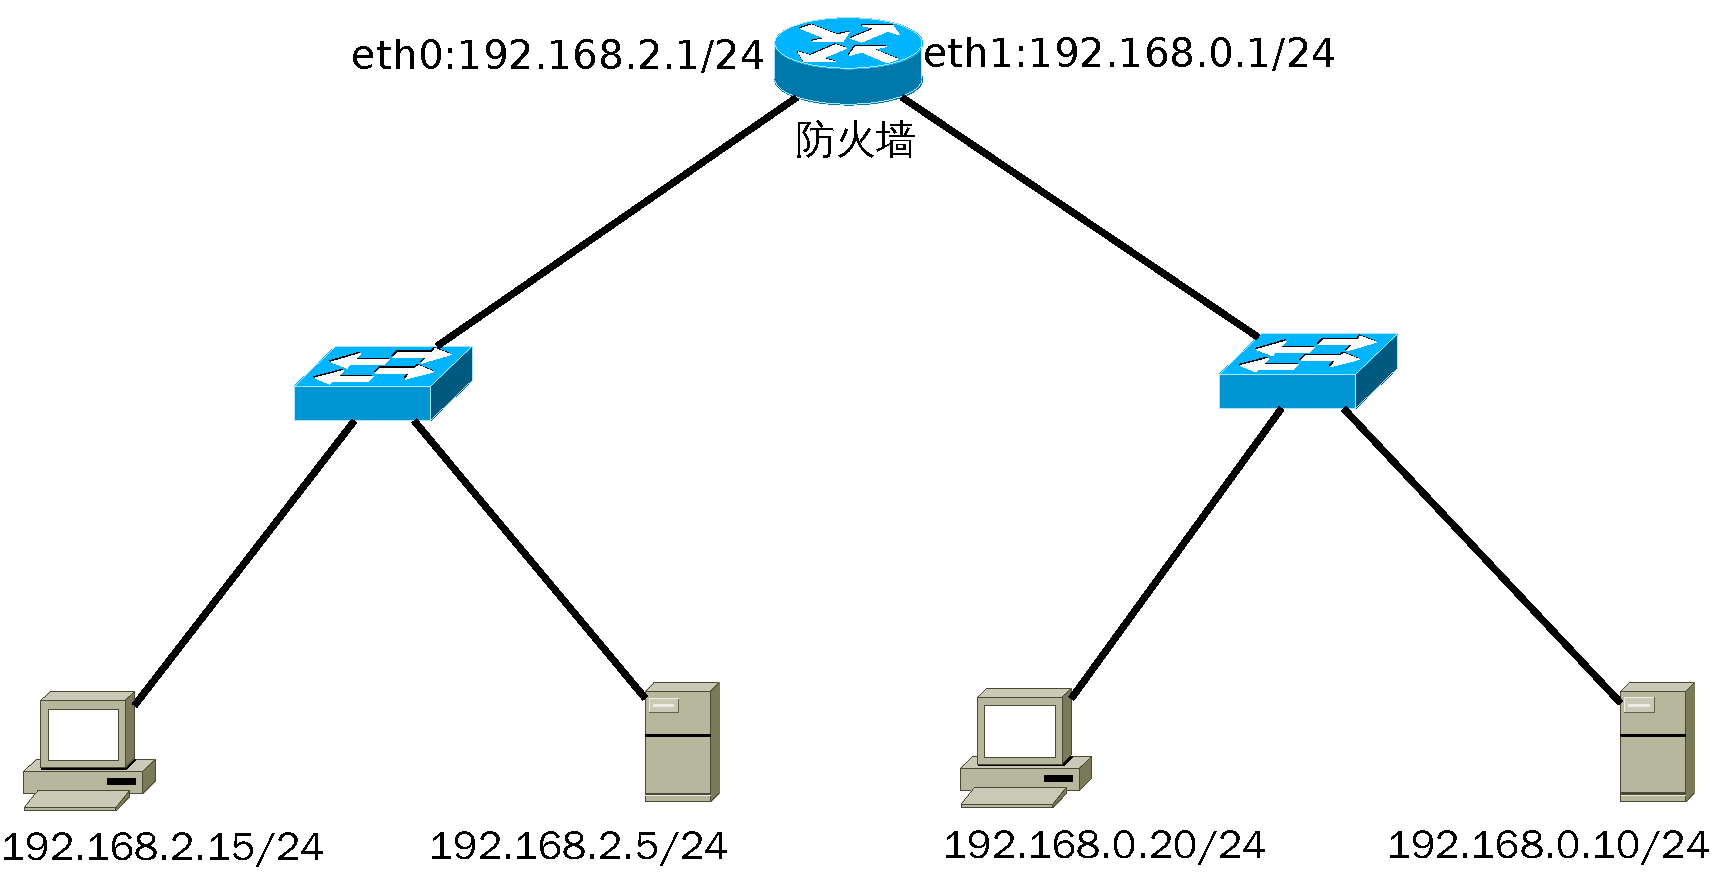
\includegraphics[width=.9\linewidth]{img/iptables-test.pdf}
\begin{itemize}

\item 2. 如果在防火墙上执行iptables -A INPUT -i eth0 -p icmp -d 192.168.0.2 -j DROP,请问192.168.2.15及192.168.0.20谁可以ping到防火墙?
\label{sec-2-30-2}%
\end{itemize} % ends low level
\end{frame}
\begin{frame}
\frametitle{iptables命令练习(3)}
\label{sec-2-31}
%% 图
\label{sec-2-31-1}

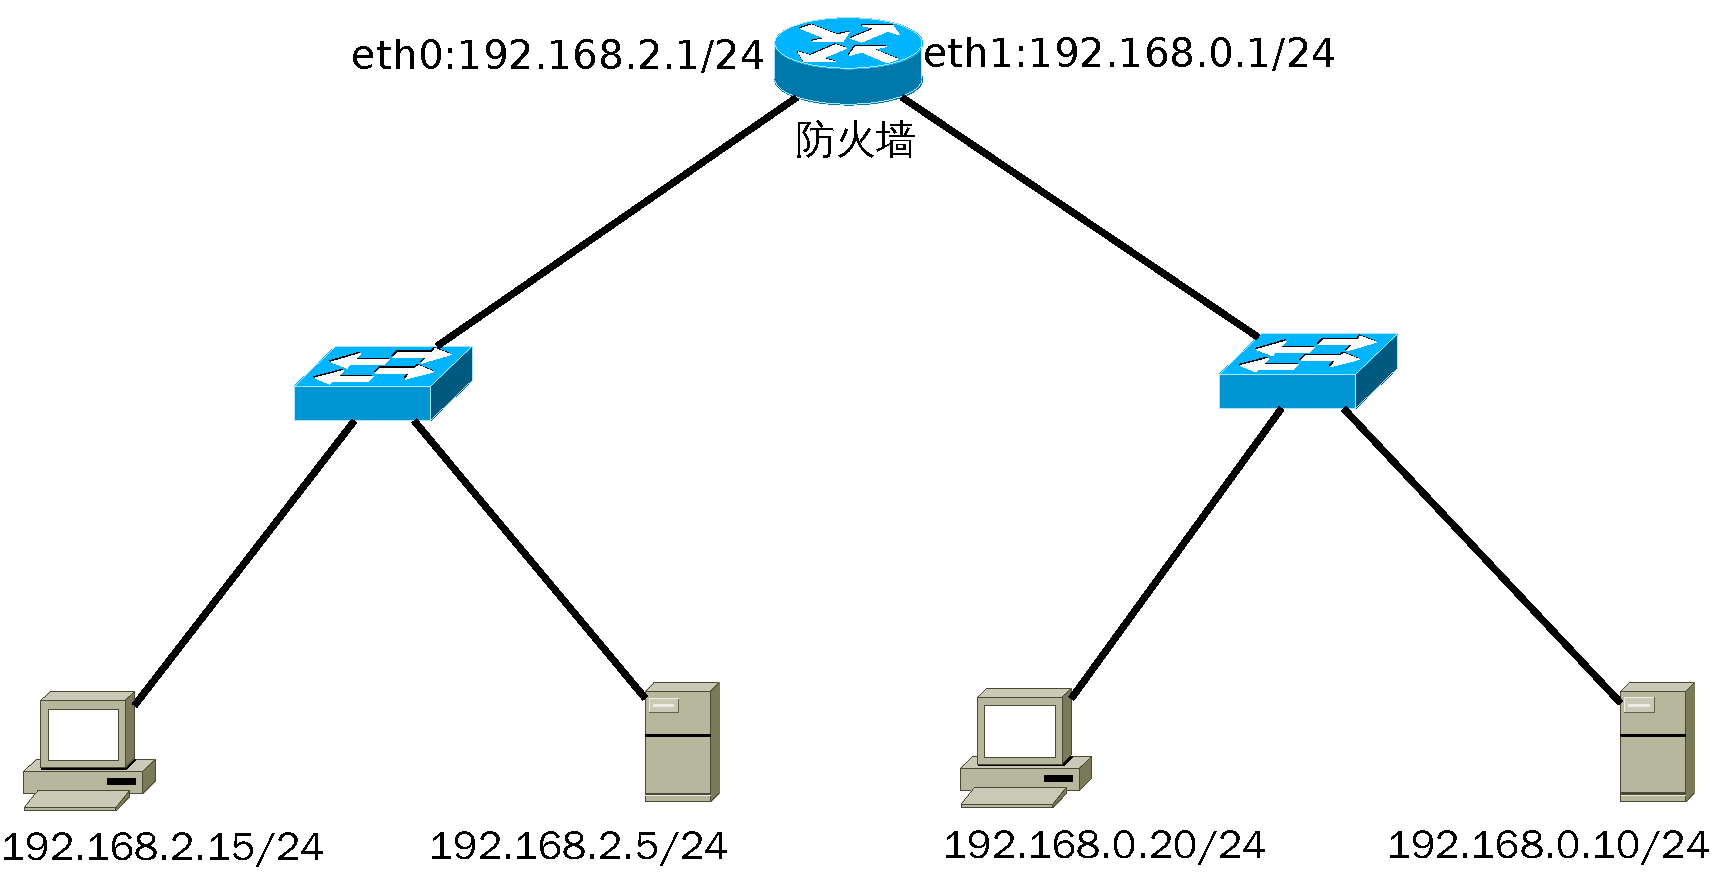
\includegraphics[width=.9\linewidth]{img/iptables-test.pdf}
\begin{itemize}

\item 3. 如果在防火墙上执行iptables -A INPUT -i eth1 --dport 80 -s 192.168.0.0/24 -j REJECT,假设防火墙上正在运行Web服务,请问哪些主机可以访问该Web服务?
\label{sec-2-31-2}%
\end{itemize} % ends low level
\end{frame}
\begin{frame}
\frametitle{iptables命令练习(4)}
\label{sec-2-32}
%% 图
\label{sec-2-32-1}

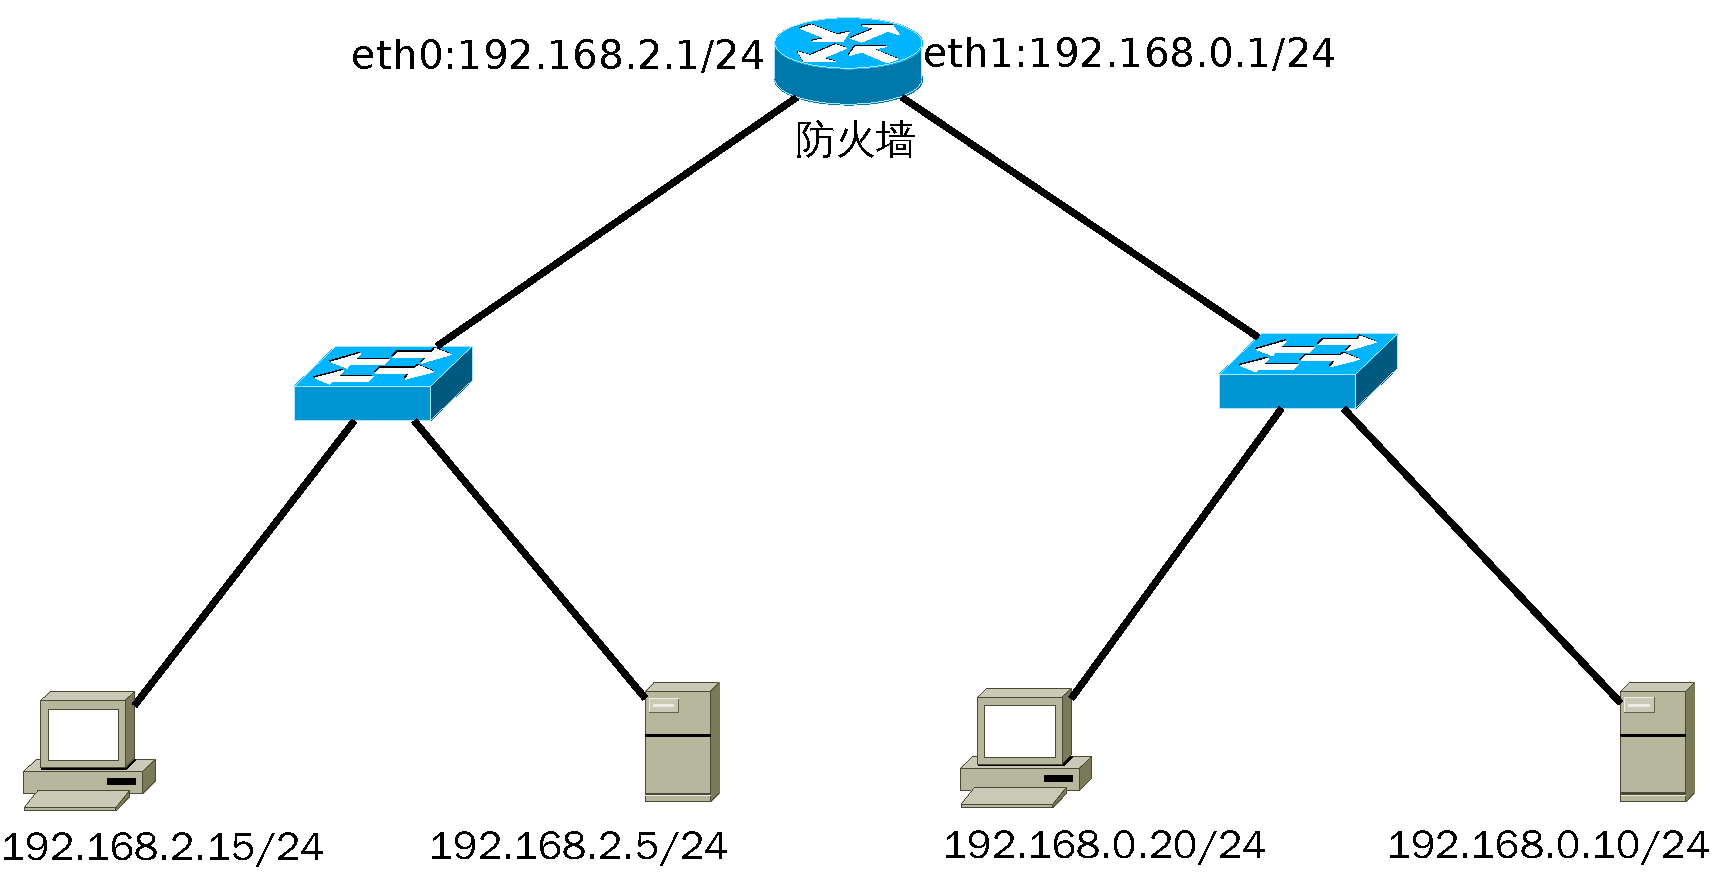
\includegraphics[width=.9\linewidth]{img/iptables-test.pdf}
\begin{itemize}

\item 4. iptables -A INPUT -i eth1 -p tcp -d 192.168.2.5 --dport 80 -j REJECT,假设192.168.2.5是Web服务器,请问192.168.2.15及192.168.0.20哪一台主机可以访问该服务器?
\label{sec-2-32-2}%
\end{itemize} % ends low level
\end{frame}
\begin{frame}
\frametitle{iptables命令练习(5)}
\label{sec-2-33}
%% 图
\label{sec-2-33-1}

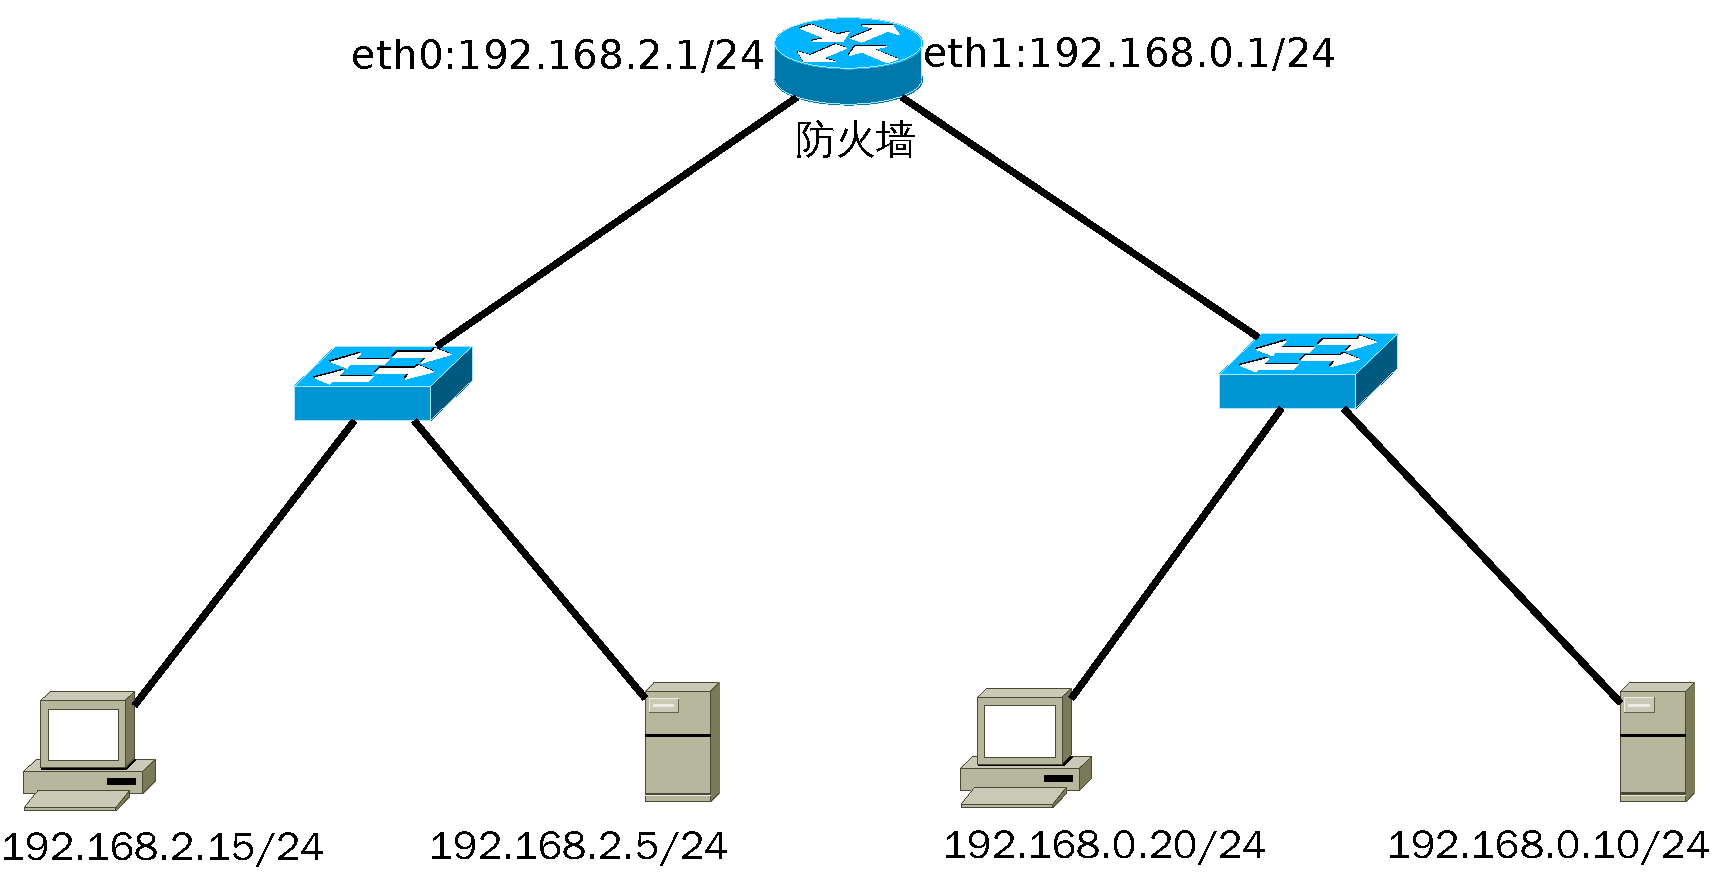
\includegraphics[width=.9\linewidth]{img/iptables-test.pdf}
\begin{itemize}

\item 5. iptables -A FORWARD -i eth0 -o eth1 -p tcp --dport 80 -j REJECT,假设192.168.2.5和192.168.0.10都是Web服务器,请问:192.168.0.20可以访问哪台Web服务器? 192.168.2.15呢?
\label{sec-2-33-2}%
\end{itemize} % ends low level
\end{frame}
\begin{frame}[fragile]
\frametitle{iptables命令的基本使用(1)}
\label{sec-2-34}
\begin{itemize}

\item 定义iptables规则的基本原则
\label{sec-2-34-1}%
\begin{itemize}

\item 通常先拒绝所有数据包,再允许部分数据包,或反之;
\label{sec-2-34-1-1}%

\item 规则尽可能简单,能用一条解决的,就不要用多条;
\label{sec-2-34-1-2}%

\item 注意规则顺序:特殊规则放前面,通用规则放后面。
\label{sec-2-34-1-3}%
\end{itemize} % ends low level

\item 保存iptables规则
\label{sec-2-34-2}%
\begin{itemize}

\item 用iptables命令创建的规则将自动保存到内存中,以root身份执行以下命令可永久保存规则:\\
\label{sec-2-34-2-1}%
\begin{minted}[]{bash}
service iptables save #保存至/etc/sysconfig/iptables
\end{minted}

\item 也可以将iptables规则保存至指定文件:\\
\label{sec-2-34-2-2}%
\begin{minted}[]{bash}
iptables-save 文件路径名
\end{minted}
\end{itemize} % ends low level

\item 管理iptables服务\\
\label{sec-2-34-3}%
\begin{minted}[]{bash}
service iptables {start|stop|restart|status|panic|save}
#panic:丢弃所有防火墙规则,所有表中的策略都被设为DROP
\end{minted}
\end{itemize} % ends low level
\end{frame}
\begin{frame}
\frametitle{iptables命令的基本使用(2)}
\label{sec-2-35}
\begin{itemize}

\item iptables控制脚本配置文件/etc/sysconfig/iptables-config
\label{sec-2-35-1}%
\begin{itemize}

\item IPTABLES\_MODULES:指定一组空间独立的额外iptables模块在激活防火墙时加载。
\label{sec-2-35-1-1}%

\item IPTARLES\_MODULES\_UNLOAD:在重新启动和停止时是否卸载模块。
\label{sec-2-35-1-2}%

\item IPTABLES\_SAVE\_ON\_STOP:停止防火墙时是否将当前的防火墙规则保存到/etc/sysconfig/iptables文件。
\label{sec-2-35-1-3}%

\item IPTABLES\_SAVE\_ON\_RESTART:当防火墙重启时是否保存当前的防火墙规则。
\label{sec-2-35-1-4}%

\item IPTABLES\_SAVE\_COUNTER:保存并恢复所有链和规则中的数据包和字节计数器。
\label{sec-2-35-1-5}%

\item IPTABLES\_STATUS\_NUMERIC:输出的IP地址是数字格式还是域名(主机名)。
\label{sec-2-35-1-6}%
\end{itemize} % ends low level
\end{itemize} % ends low level
\end{frame}
\section{部署iptables防火墙}
\label{sec-3}
\begin{frame}
\frametitle{iptables防火墙基本配置(1)}
\label{sec-3-1}
\begin{itemize}

\item 1. 配置网络环境\\
\label{sec-3-1-1}%
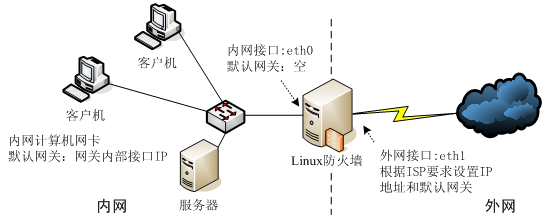
\includegraphics[width=.9\linewidth]{img/iptables7.png}
\end{itemize} % ends low level
\end{frame}
\begin{frame}[fragile]
\frametitle{iptables防火墙基本配置(2)}
\label{sec-3-2}
\begin{itemize}

\item 2. 清除原有规则和计数器\\
\label{sec-3-2-1}%
\begin{minted}[]{bash}
iptables -F; iptables -X; iptables -Z
iptables -t nat -F
iptables -t nat -X
iptables -t nat -Z
\end{minted}

\item 3. 设置默认策略\\
\label{sec-3-2-2}%
\begin{minted}[]{bash}
iptables -P INPUT DROP
iptables -P FORWARD DROP
iptables -P OUTPUT DROP
iptables -t nat -P PREROUTING ACCEPT
iptables -t nat -P OUTPUT ACCEPT
iptables -t nat -P POSTROUTING ACCEPT
\end{minted}

\item 3. 保存规则并启用\\
\label{sec-3-2-3}%
\begin{minted}[]{bash}
service iptables save; service iptables restart
\end{minted}
\end{itemize} % ends low level
\end{frame}
\begin{frame}[fragile]
\frametitle{在防火墙上开放必要的内外网间通信}
\label{sec-3-3}
\begin{itemize}

\item 1. 允许回环地址通信\\
\label{sec-3-3-1}%
\begin{minted}[]{bash}
iptables -I INPUT 1 -i lo -j ACCEPT
iptables -I OUTPUT 1 -o lo -j ACCEPT
\end{minted}

\item 2. 开放防火墙上的端口\\
\label{sec-3-3-2}%
\begin{minted}[]{bash}
iptables -A INPUT -p tcp --dport 80 -j ACCEPT
iptables -A OUTPUT -p tcp --sport 80 -j ACCEPT
\end{minted}

\item 3. 允许通过SSH管理防火墙\\
\label{sec-3-3-3}%
\begin{minted}[]{bash}
iptables -A INPUT -p tcp --dport 22 -j ACCEPT
iptables -A OUTPUT -p tcp --sport 22 -j ACCEPT
#以下命令仅允许从外网(eth1)访问防火墙
iptables -A INPUT -p tcp -i eth1 --dport 22 -j ACCEPT
iptables -A OUTPUT -p tcp -o eth1 --sport 22 -j ACCEPT
\end{minted}
\end{itemize} % ends low level
\end{frame}
\begin{frame}[fragile]
\frametitle{通过NAT方式共享上网(1)}
\label{sec-3-4}
\begin{itemize}

\item 1. 服务器端NAT设置(1)
\label{sec-3-4-1}%
\begin{itemize}

\item 可通过定义nat表的POSTROUTING链来实现共享网络连接。一般为防火墙配置IP伪装(MASQUERADE),将发出请求的内网节点地址转换为防火墙设备(例中为eth1):\\
\label{sec-3-4-1-1}%
\begin{minted}[]{bash}
iptables -t nat -A POSTROUTING -o eth1 -j MASQUERADE
\end{minted}

\item IP伪装适合动态源地址转换,如果防火墙外网接口使用动态IP地址(例如采用拨号方式或DHCP接入Internet),必须使用MASQUERADE方式:\\
\label{sec-3-4-1-2}%
\begin{minted}[]{bash}
iptables -t nat -A POSTROUTING -o ppp0 -j MASQUERADE
\end{minted}
\end{itemize} % ends low level
\end{itemize} % ends low level
\end{frame}
\begin{frame}[fragile]
\frametitle{通过NAT方式共享上网(2)}
\label{sec-3-5}
\begin{itemize}

\item 1. 服务器端NAT设置(2)
\label{sec-3-5-1}%
\begin{itemize}

\item 源NAT(SNAT)和IP伪装都可以实现多台主机共享一个Internet连接,作用是一样的。如果防火墙外网接口使用静态IP地址,可以直接使用源NAT方式,定义如下:\\
\label{sec-3-5-1-1}%
\begin{minted}[]{bash}
iptables -t nat -A POSTROUTING -o eth1 \
-j SNAT --to 172.16.0.10
\end{minted}

\item 还可以进一步限制共享连接的内网地址,例如:\\
\label{sec-3-5-1-2}%
\begin{minted}[]{bash}
iptables -t nat -A POSTROUTING -o eth1 \
-s 192.168.0.0/24 -j MASQUERADE
\end{minted}
\end{itemize} % ends low level
\end{itemize} % ends low level
\end{frame}
\begin{frame}[fragile]
\frametitle{通过NAT方式共享上网(3)}
\label{sec-3-6}
\begin{itemize}

\item 2. 调整防火墙包转发规则
\label{sec-3-6-1}%
\begin{itemize}

\item 简单方法:将FORWARD链的默认策略该为允许\\
\label{sec-3-6-1-1}%
\begin{minted}[]{bash}
iptables -P FORWARD ACCEPT
\end{minted}

\item 规范方法:保留DROP默认策略,添加相应允许规则\\
\label{sec-3-6-1-2}%
\begin{minted}[]{bash}
#允许为整个内网(eth0)转发分组
iptables -A FORWARD -i eth0 -j ACCEPT
iptables -A FORWARD -o eth0 -j ACCEPT
\end{minted}

\item 可根据需要设置仅允许转发特定协议的包,如DNS和HTTP:\\
\label{sec-3-6-1-3}%
\begin{minted}[]{bash}
iptables -A FORWARD -p tcp --dport 53 -j ACCEPT
iptables -A FORWARD -p tcp --sport 53 -j ACCEPT
iptables -A FORWARD -p udp --dport 53 -j ACCEPT
iptables -A FORWARD -p udp --sport 53 -j ACCEPT
iptables -A FORWARD -p tcp --dport 80 -j ACCEPT
iptables -A FORWARD -p tcp --sport 80 -j ACCEPT
\end{minted}
\end{itemize} % ends low level
\end{itemize} % ends low level
\end{frame}
\begin{frame}
\frametitle{通过NAT方式共享上网(4)}
\label{sec-3-7}
\begin{itemize}

\item 3. 客户端NAT设置
\label{sec-3-7-1}%
\begin{itemize}

\item 只要设置NAT客户端的默认网关为NAT服务器eth0的IP地址,DNS设为ISP的DNS服务器就可上网了。
\label{sec-3-7-1-1}%
\end{itemize} % ends low level
\end{itemize} % ends low level
\end{frame}
\begin{frame}[fragile]
\frametitle{通过端口映射发布内网服务器(1)}
\label{sec-3-8}
\begin{itemize}

\item 1. 定义NAT端口映射
\label{sec-3-8-1}%
\begin{itemize}

\item 可以使用nat表的PREROUTING链的-j DNAT目标来定义转发传入数据包(请求连接到内网服务)的目标IP地址或端口。\\
\label{sec-3-8-1-1}%
\begin{minted}[]{bash}
iptables -t nat -A PREROUTING -i eth1 \
-p tcp --dport 80 -j DNAT --to 192.168.0.1:80
\end{minted}
\end{itemize} % ends low level

\item 2. 调整包转发规则
\label{sec-3-8-2}%
\begin{itemize}

\item 如果定义FORWARD链的“DROP”默认策略,可使用以下规则(防火墙内网接口为eth0)允许为内外网之间转发包。\\
\label{sec-3-8-2-1}%
\begin{minted}[]{bash}
iptables -A FORWARD -i eth0 -j ACCEPT
iptables -A FORWARD -o eth0 -j ACCEPT
\end{minted}

\item 如果只转发传入HTTP请求,可将规则修改为:\\
\label{sec-3-8-2-2}%
\begin{minted}[]{bash}
iptables -A FORWARD -i eth1 -p tcp --dport 80 \
-d 192.168.0.1 -j ACCEPT
iptables -A FORWARD -o eth1 -p tcp --sport 80 \
-s 192.168.0.1 -j ACCEPT
\end{minted}
\end{itemize} % ends low level
\end{itemize} % ends low level
\end{frame}
\begin{frame}[fragile]
\frametitle{通过端口映射发布内网服务器(2)}
\label{sec-3-9}
\begin{itemize}

\item 发布多台Web服务器
\label{sec-3-9-1}%
\begin{itemize}

\item 可在防火墙上利用多端口发布多个Web服务器。例如:\\
\label{sec-3-9-1-1}%
\begin{minted}[]{bash}
iptables -t nat -A PREROUTING -i eth1 -p tcp \
--dport 80 -j DNAT --to 192.168.0.1:80
iptables -t nat -A PREROUTING -i eth1 -p tcp \
--dport 8000 -j DNAT --to 192.168.0.20:80
\end{minted}
\end{itemize} % ends low level

\item 发布其他服务器
\label{sec-3-9-2}%
\begin{itemize}

\item 以FTP服务器为例,使用以下规则:\\
\label{sec-3-9-2-1}%
\begin{minted}[]{bash}
iptables -t nat -A PREROUTING -i eth1 -p tcp \
--dport 20 -j DNAT --to 192.168.0.1:20
iptables -t nat -A PREROUTING -i eth1 -p tcp \
--dport 21 -j DNAT --to 192.168.0.1:21
\end{minted}
\end{itemize} % ends low level
\end{itemize} % ends low level
\end{frame}
\begin{frame}[fragile]
\frametitle{防止恶意软件和假冒IP地址}
\label{sec-3-10}
\begin{itemize}

\item 可以限制访问服务器带来的恶意应用程序,如木马、蠕虫和其他客户/服务器病毒。例如,一些木马在端口31337\~{}31340(黑客术语称为“elite”端口)扫描网络服务。以下规则丢弃试图使用31337端口的所有TCP数据包:\\
\label{sec-3-10-1}%
\begin{minted}[]{bash}
iptables -A OUTPUT -o eth1 -p tcp \
--dport 31337 --sport 31337 -j DROP
iptables -A FORWARD -o eth1 -p tcp \
--dport 31337 --sport 31337 -j DROP
\end{minted}

\item 也可阻断试图仿冒内网IP地址攻击内网的外部连接。例如,如果内网用户使用192.168.0.0/24网段,可以设计一条规则指示外网接口(如eth1)丢弃到达该接口的数据包(由内网IP段的私有IP发出)\\
\label{sec-3-10-2}%
\begin{minted}[]{bash}
iptables -A FORWARD -s 192.168.0.0/24 -i eth1 -j DROP
\end{minted}

\item 如果将拒绝转发数据包作为默认策略,任何到外部设备的假冒IP地址自动被拒绝。
\label{sec-3-10-3}%
\end{itemize} % ends low level
\end{frame}
\begin{frame}[fragile]
\frametitle{配置状态防火墙}
\label{sec-3-11}
\begin{itemize}

\item 连接跟踪可以让Netfilter获知某个特定连接的状态。
\label{sec-3-11-1}%

\item iptables可设置以下4种连接状态:
\label{sec-3-11-2}%
\begin{enumerate}
\item NEW:表示匹配的数据包正在创建一个新连接
\item ESTABLISHED:表示匹配的数据包属于某个已经建立的双向传送的连接
\item RELATED:表示匹配的数据包正在启动一个与现有连接相关的新连接
\item INVALID:表示匹配的数据包不能与一个已知的连接相关联,通常应丢掉
\end{enumerate}

\item 状态匹配由state模块提供,使用时需要使用选项-m加载,以下例子表示,通过连接跟踪仅转发同已建立连接相关的数据包,如FTP-DATA数据连接:\\
\label{sec-3-11-3}%
\begin{minted}[]{bash}
iptables -A FORWARD -m state \
--state ESTABLISHED,RELATED -j ACCEPT
\end{minted}
\end{itemize} % ends low level
\end{frame}
\begin{frame}[fragile]
\frametitle{配置非军事区(DMZ)}
\label{sec-3-12}
\begin{itemize}

\item DMZ是一个非安全系统与安全系统之间的缓冲区,缓冲区位于内外网之间的特殊子网,可部署一些要公开的服务器。
\label{sec-3-12-1}%

\item 需创建iptables规则,将数据包路由到位于DMZ的服务器。
\label{sec-3-12-2}%

\item 例如,将HTTP请求路由到HTTP服务器10.0.0.2(位于内网192.168.1.0/24的外面):\\
\label{sec-3-12-3}%
\begin{minted}[]{bash}
iptables -t nat -A PREROUTING -i eth1 -p tcp \
--dport 80 -j DNAT --to-destination 10.0.0.2:80
\end{minted}

\item 如果HTTP服务器配置为接收SSL安全连接,端口443也必须转发:\\
\label{sec-3-12-4}%
\begin{minted}[]{bash}
iptables -t nat -A PREROUTING -i eth1 -p tcp \
--dport 443 -j DNAT --to-destination 10.0.0.2:80
\end{minted}
\end{itemize} % ends low level
\end{frame}
\section{部署Squid代理服务器}
\label{sec-4}
\begin{frame}[fragile]
\frametitle{安装和管理squid服务}
\label{sec-4-1}
\begin{itemize}

\item 安装squid软件包\\
\label{sec-4-1-1}%
\begin{minted}[]{bash}
yun install squid
\end{minted}

\item 管理squid服务\\
\label{sec-4-1-2}%
\begin{minted}[]{bash}
service squid {start|stop|status|reload|restart|\
condrestart}
\end{minted}
\end{itemize} % ends low level
\end{frame}
\begin{frame}[fragile]
\frametitle{squid配置文件/etc/squid/squid.conf(1)}
\label{sec-4-2}
\begin{itemize}

\item 认证选项
\label{sec-4-2-1}%
\begin{itemize}

\item Squid支持多种用户认证模式,如基本、摘要(Digest)、NTLM和协商(Negotiate),指定如何从客户端接受用户名和密码。指令auth$_{\mathrm{param}}$用于定义不同认证模式的参数:\\
\label{sec-4-2-1-1}%
\begin{minted}[]{bash}
auth_param 模式 参数 [设置]
\end{minted}
\end{itemize} % ends low level

\item 访问控制选项
\label{sec-4-2-2}%
\begin{itemize}

\item Squid默认拒绝所有访问客户端的请求,为了能让客户端通过代理服务器访问,最简单的方法就是定义一个针对客户端IP地址的访问控制列表(ACL),并允许来自这些地址的HTTP请求。\\
\label{sec-4-2-2-1}%
\begin{minted}[]{bash}
acl 访问控制列表名称 访问控制列表类型 字符串1 ...
http_access allow|deny [!]访问控制列表名称 ...
\end{minted}
\end{itemize} % ends low level

\item 网络选项
\label{sec-4-2-3}%
\begin{itemize}

\item 网络选项http$_{\mathrm{port}}$指定Squid监听客户端HTTP请求的IP地址和端口,语法格式为:\\
\label{sec-4-2-3-1}%
\begin{minted}[]{bash}
http_port [主机名或IP:] 端口 [选项]
\end{minted}
\end{itemize} % ends low level
\end{itemize} % ends low level
\end{frame}
\begin{frame}[fragile]
\frametitle{squid配置文件/etc/squid/squid.conf(2)}
\label{sec-4-3}
\begin{itemize}

\item 相邻缓存服务器选项:用于设置多层缓存\\
\label{sec-4-3-1}%
\begin{minted}[]{bash}
#指定多层缓存网络中其他缓存服务器
cache_peer hostname type http_port icp_port [options]
cache_peer p.abc.com parent 3128 3130 proxy-only default
cache_peer s1.abc.com sibling 3128 3130 proxy-only
cache_peer s2.abc.com sibling 3128 3130 proxy-only
#type: parent(父级)、sibling(同级)
#http_port: 该缓存服务器监听客户端http请求的端口,默认3128
#icp_port:该缓存服务器ICP查询所用端口,默认3130
#options:proxy-only:不保存来自缓存的对象
#         default:作为顶层缓存服务器
#限定要查询的邻居缓存服务器的域
cache_peer_domain p.abc.com [!].edu
#通过acl提供更灵活的访问控制
cache_peer_access p.abc.com allow|deny acl1
\end{minted}
\end{itemize} % ends low level
\end{frame}
\begin{frame}[fragile]
\frametitle{squid配置文件/etc/squid/squid.conf(3)}
\label{sec-4-4}
\begin{itemize}

\item 内存缓存选项\\
\label{sec-4-4-1}%
\begin{minted}[]{bash}
cache_mem 8 MB #squid可以使用的内存大小
#内存缓存中可保存的最大对象
maximum_object_size_in_memory 8KB
\end{minted}

\item 硬盘缓存选项\\
\label{sec-4-4-2}%
\begin{minted}[]{bash}
#指定缓存空间的类型,位置,大小及其目录结构
cache_dir ufs /var/spool/squid 100 16 256
cache_swap_low 90  #交换空间上限
cache_swap_high 95 #交换空间下限
maximum_object_size 4096KB #硬盘缓存中可保存的最大对象
\end{minted}
\end{itemize} % ends low level
\end{frame}
\begin{frame}
\frametitle{squid配置文件/etc/squid/squid.conf(4)}
\label{sec-4-5}
\begin{itemize}

\item 日志文件路径
\label{sec-4-5-1}%
\begin{itemize}

\item logformat:定义访问日志文件格式
\label{sec-4-5-1-1}%

\item access\_log:设置记录客户请求的日志文件
\label{sec-4-5-1-2}%

\item cache\_log:设置squid产生的一般信息的日志文件
\label{sec-4-5-1-3}%

\item cache\_store\_log:设置记录对象存储情况的日志文件
\label{sec-4-5-1-4}%
\end{itemize} % ends low level

\item 管理参数
\label{sec-4-5-2}%
\begin{itemize}

\item cache\_mgr:设置管理员的邮件地址
\label{sec-4-5-2-1}%

\item cache\_effective\_user与cache\_effective\_group:设置squid启动后,以何用户身份运行,默认设置为squid
\label{sec-4-5-2-2}%

\item visible\_hostname:定义在返回给用户的出错信息中所显示的主机名
\label{sec-4-5-2-3}%
\end{itemize} % ends low level
\end{itemize} % ends low level
\end{frame}
\begin{frame}
\frametitle{squid配置文件/etc/squid/squid.conf(5)}
\label{sec-4-6}
\begin{itemize}

\item 超时设置
\label{sec-4-6-1}%
\begin{itemize}

\item connect\_timeout:设置Squid等待连接完成的超时值,默认为1分钟
\label{sec-4-6-1-1}%

\item peer\_connect\_timeout:设置连接其他缓存服务器的超时值,默认为30秒
\label{sec-4-6-1-2}%

\item read\_timeout:如果客户在指定时间内,未从Squid服务器读取任何数据,则Squid将终止该客户的请求,默认为15分钟
\label{sec-4-6-1-3}%

\item request\_timeout:设置Squid与客户端建立连接后,等待客户发出HTTP请求的超时时间,默认设置为5分种
\label{sec-4-6-1-4}%

\item persistent\_request\_timeout:设置在前一个连接请求完成后,在同一个连接上等待下一个新的HTTP请求的超时时间,默认设置为1分钟
\label{sec-4-6-1-5}%

\item ident\_timeout:设置Squid等待用户认证请求的超时时间,默认为10秒
\label{sec-4-6-1-6}%
\end{itemize} % ends low level
\end{itemize} % ends low level
\end{frame}
\begin{frame}[fragile]
\frametitle{squid命令行}
\label{sec-4-7}
\begin{itemize}

\item squid命令可用于管理和调试,主要选项如下
\label{sec-4-7-1}%
\begin{itemize}

\item -f file:用指定配置文件取代默认配置文件
\label{sec-4-7-1-1}%

\item -k:让squid执行指定管理功能\\
\label{sec-4-7-1-2}%
\begin{minted}[]{bash}
reconfigure #重新读取配置文件
shutdown    #关闭
debug       #进入调试模式
check       #检查squid进程
parse       #检查配置文件
\end{minted}

\item -u port:指定ICP端口号,取代配置文件内的icp\_port
\label{sec-4-7-1-3}%

\item -z:初始化缓存,首次运行squid或者增加新的缓存目录时,必须使用该选项!
\label{sec-4-7-1-4}%
\end{itemize} % ends low level
\end{itemize} % ends low level
\end{frame}
\begin{frame}[fragile]
\frametitle{配置标准代理服务器(1)}
\label{sec-4-8}


\begin{minted}[]{bash}
vim /etc/squid/squid.conf
http_port 192.168.0.2:3128 #监听地址及端口
cache_mem 128 MB #设置高速缓存为128MB
cache_dir ufs /var/spool/squid 4096 16 256 #设置硬盘缓存
access_log /var/log/squid/access.log #设置访问日志
cache_log /var/log/squid/cache.log #设置缓存日志
cache_store_log /var/log/squid/store.log #设置网页缓存日志
dns_nameservers 211.137.191.26 #设置DNS服务器
acl all src 0.0.0.0/0.0.0.0 #定义访问控制列表all
http_access allow all #允许所有客户端访问
cache_mgr root@abc.com #设置管理员E-mail地址
cache_effective_user squid #设置squid进程所有者
cache_effective_group squid #设置squid进程所属组
visible_hostname 192.168.0.2 #设置squid可见主机名
\end{minted}
\end{frame}
\begin{frame}[fragile]
\frametitle{配置标准代理服务器(2)}
\label{sec-4-9}
\begin{itemize}

\item 如果Linux服务器开启了防火墙功能,还需要关闭防火墙功能,或者允许访问代理服务器端口(例中为3128。\\
\label{sec-4-9-1}%
\begin{minted}[]{bash}
iptables -A INPUT -p tcp --dport 3128 -j ACCEPT
\end{minted}

\item 配置代理客户端
\label{sec-4-9-2}%
\begin{itemize}

\item 打开Firefox浏览器中,选择“编辑”>“首选项”菜单打开相应的对话框,在“常规”选项卡中单击“连接设置”按钮,然后选中“手动配置代理”单选钮,在“HTTP代理”和“端口”文本框中输入要使用的代理服务器的IP地址及端口号。
\label{sec-4-9-2-1}%

\item Windows平台上一般使用IE浏览器。打开IE浏览器,选择“工具”>“Internet选项”菜单打开相应的对话框,切换到“连接”选项卡,单击“局域网设置”按钮,然后选中“为LAN使用代理服务器”复选框,输入代理服务器正确的IP地址及端口号。
\label{sec-4-9-2-2}%
\end{itemize} % ends low level
\end{itemize} % ends low level
\end{frame}
\begin{frame}[fragile]
\frametitle{squid服务器访问控制(1)}
\label{sec-4-10}
\begin{itemize}

\item 允许某内部网段用户访问\\
\label{sec-4-10-1}%
\begin{minted}[]{bash}
acl mynet src 192.168.0.0/255.255.0.0
http_access allow mynet
http_access deny all
\end{minted}

\item 禁止某内部网段用户访问\\
\label{sec-4-10-2}%
\begin{minted}[]{bash}
acl othernet src 192.168.10.0/255.255.0.0
http_access deny othernet
\end{minted}

\item 站点屏蔽\\
\label{sec-4-10-3}%
屏蔽某些特定站点或含有某些特定字词的站点,例如:

\begin{minted}[]{bash}
acl sexurl url-regex -i sex
http_access deny sexurl
\end{minted}
\end{itemize} % ends low level
\end{frame}
\begin{frame}[fragile]
\frametitle{squid服务器访问控制(2)}
\label{sec-4-11}
\begin{itemize}

\item 下载内容屏蔽\\
\label{sec-4-11-1}%
禁止客户机下载*.mp3、*.exe、*.zip和*.rar类型的文件。

\begin{minted}[]{bash}
ac1 bigfiles urlpath_regex -i \.mp3$ \.exe$ \zip$ \.rar$
http_access deny bigfiles
\end{minted}

\item 限制访问时段\\
\label{sec-4-11-2}%
允许所有用户在周一至周五8:30\~{}20:30访问代理服务器,允许管理员每天下午访问代理服务器,其他时段一律拒绝访问。

\begin{minted}[]{bash}
act all src 0.0.0.0/0.0.0.0
acl administrator 192.168.0.0/24
acl common_time time MTWHF 8:30-20:30
acl manage_time time MTWHFAS 13:00-18:00
http_access allow all common_time
http_access allow administrator manage_time
http_access deny all
\end{minted}
\end{itemize} % ends low level
\end{frame}
\begin{frame}[fragile]
\frametitle{squid服务器访问控制(3)}
\label{sec-4-12}
\begin{itemize}

\item 设置CONNECT\\
\label{sec-4-12-1}%
有些用户通过二级代理软件访问非法站点,可在Squid中通过CONNECT方法来拒绝访问。

\begin{minted}[]{bash}
acl all src 0.0.0.0/0.0.0.0
acl manager proto cache_object
acl localhost src 127.0.0.1/255.255.255.255
acl to_localhost dst 127.0.0.0/8
acl SSL_ports port 443
acl Safe_ports port 80 # http
acl Safe_ports port 21 # ftp
acl Safe_ports port 443 # https
acl Safe_ports port 1025-65535 # unregistered ports
acl Safe_ports port 777 # multiling http
acl CONNECT method CONNECT
\end{minted}
\end{itemize} % ends low level
\end{frame}
\begin{frame}[fragile]
\frametitle{squid服务器访问控制(4)}
\label{sec-4-13}
\begin{itemize}

\item 设置CONNECT(续)\\
\label{sec-4-13-1}%
\begin{minted}[]{bash}
http_access allow manager localhost
http_access deny manager
http_access deny !Safe_ports
http_access deny CONNECT !SSL_ports
\end{minted}




\end{itemize} % ends low level
\end{frame}
\begin{frame}[fragile]
\frametitle{squid服务器用户认证(1)}
\label{sec-4-14}
\begin{itemize}

\item 在Squid配置文件中设置认证选项
\label{sec-4-14-1}%
\begin{itemize}

\item (1)设置要使用的认证程序及其相关选项,在配置文件开头部分设置以下选项。\\
\label{sec-4-14-1-1}%
\begin{minted}[]{bash}
# 定义认证方式、认证程序路径和需读取的账户文件
auth_param basic program \
/usr/lib/squid/ncsa_auth /etc/squid/passwd
# 设置认证程序的进程数
auth_param basic children 5
# 设置认证有效时间,超过该时间要求重新输入用户名和密码
auth_param basic credentialsttl 2 hours
# 设置认证领域内容,即浏览器显示认证对话框时的提示内容
auth_param basic realm \
This is a Squid proxy-caching
\end{minted}
\end{itemize} % ends low level
\end{itemize} % ends low level
\end{frame}
\begin{frame}[fragile]
\frametitle{squid服务器用户认证(2)}
\label{sec-4-15}
\begin{itemize}

\item 在Squid配置文件中设置认证选项(续)
\label{sec-4-15-1}%
\begin{itemize}

\item (2)为认证用户设置ACL,并给出访问控制规则,在配置文件中设置以下选项。\\
\label{sec-4-15-1-1}%
\begin{minted}[]{bash}
acl noauth_user src 192.168.0.21
acl auth_user proxy_auth REQUIRED
http_access allow noauth_user
http_access allow auth_user
\end{minted}
\end{itemize} % ends low level
\end{itemize} % ends low level
\end{frame}
\begin{frame}[fragile]
\frametitle{squid服务器用户认证(3)}
\label{sec-4-16}
\begin{itemize}

\item 建立账户文件
\label{sec-4-16-1}%
\begin{itemize}

\item 为建立供用户认证使用的账户文件,可利用Apache的htpasswd程序生成账户文件/etc/squid/passwd,该账户文件每行包含一个用户的信息,即用户名和经过加密后的密码。\\
\label{sec-4-16-1-1}%
\begin{minted}[]{bash}
htpasswd -c /etc/squid/passwd mike #添加首个用户
htpasswd /etc/squid/passwd mary #添加后续用户

service squid restart
\end{minted}

\item 测试用户认证
\label{sec-4-16-1-2}%
\begin{itemize}

\item 重启squid服务
\label{sec-4-16-1-2-1}%

\item 配置客户端
\label{sec-4-16-1-2-2}%

\item 测试访问网页
\label{sec-4-16-1-2-3}%
\end{itemize} % ends low level

\item 注意:squid不支持在透明代理模式下启用用户身份认证功能,但在正、反向代理模式下都有效。
\label{sec-4-16-1-3}%
\end{itemize} % ends low level
\end{itemize} % ends low level
\end{frame}
\begin{frame}
\frametitle{配置透明代理服务器(1)}
\label{sec-4-17}
\begin{itemize}

\item 概述
\label{sec-4-17-1}%
\begin{itemize}

\item 所谓透明,是指客户端感觉不到代理的存在,不需要对浏览器进行代理设置。
\label{sec-4-17-1-1}%

\item 在squid中,透明代理又称Interception Caching(拦截缓存),或缓存重定向。
\label{sec-4-17-1-2}%

\item 透明代理服务器阻断网络通信,并且过滤出访问外网的HTTP(80端口)流量。如果客户端的请求在本地有缓存,则将缓存的数据直接发给用户。
\label{sec-4-17-1-3}%

\item 对于Linux服务器来说,将iptables与Squid服务器结合起来可实现这种透明代理。Squid支持HTTP和FTP等协议的代理,在缓存数据的同时,也缓存DNS查询结果,支持SSL和访问控制;对于Squid无法代理的服务,则可通过iptables共享连接来实现,同时具有缓存功能,加速Web的访问。
\label{sec-4-17-1-4}%
\end{itemize} % ends low level
\end{itemize} % ends low level
\end{frame}
\begin{frame}[fragile]
\frametitle{配置透明代理服务器(2)}
\label{sec-4-18}
\begin{itemize}

\item 透明代理配置过程\\
\label{sec-4-18-1}%
\begin{minted}[]{bash}
#1. 修改squid.conf,启用透明代理支持
http_port 192.168.0.2:3128 transparent
#2. 启用ip转发功能
#3. 配置iptables,实现http流量拦截
iptables -t nat -A PREROUTING -i eth0 -p tcp \
--dport 80 -j REDIRECT --to-ports 3128
iptables -t nat -A POSTROUTING -o eth1 -j MASQUERADE
#4. 重启squid或重新加载squid配置文件
#5. 重启iptables
#6. 客户端只需要将默认网关设置为squid主机的内网地址,
#   即可正常访问外部网站
\end{minted}
\end{itemize} % ends low level
\end{frame}
\begin{frame}[fragile]
\frametitle{配置反向代理服务器(1)}
\label{sec-4-19}
\begin{itemize}

\item 配置基本的反向代理服务器
\label{sec-4-19-1}%
\begin{itemize}

\item 关于反向代理的选项必须出现在squid.conf配置文件开头,在其他转发代理配置(如http$_{\mathrm{access}}$等)之前,否则标准代理访问规则将阻止访问加速站点(反向代理服务器)。\\
\label{sec-4-19-1-1}%
\begin{minted}[]{bash}
#设置反向代理监听端口(通常为80)和反向代理模式
http_port 80 accel
#设置所代理的内部web服务器
cache_peer 192.168.0.21 parent 80 0 \
no-query originserver name=myAccel
#设置允许访问该加速站点,不允许其他访问
acl our_sites dstdomain www.abc.name
http_access allow our_sites
cache_peer_access myAccel allow our_sites
cache_peer_access myAccel deny all
#重启squid服务
#将web网站的公共域名执行squid服务器后进行访问测试
\end{minted}
\end{itemize} % ends low level
\end{itemize} % ends low level
\end{frame}
\begin{frame}[fragile]
\frametitle{配置反向代理服务器(2)}
\label{sec-4-20}
\begin{itemize}

\item 多台服务器配置
\label{sec-4-20-1}%
\begin{itemize}

\item 例:两台内网服务器(192.168.0.2和192.168.0.21),squid的内网接口eth0(192.168.0.2),外网接口eth1(172.16.0.10)。\\
\label{sec-4-20-1-1}%
\begin{minted}[]{bash}
http_port 80 vhost #设置监听端口,并启用反向代理
#指定Squid要代理的内部Web服务器
cache_peer 192.168.0.2 parent 80 0 \
no-query originserver name=a
cache_peer 192.168.0.21 parent 80 0 \
no-query originserver name=b
cache_peer_domain a www.servera.com
cache_peer_domain b www.serverb.com
#设置访问控制,允许所有外部客户端访问这些站点
acl all src 0.0.0.0/0.0.0.0
http_access allow all
cache_peer_access a allow all
cache_peer_access b allow all
#重启squid,将公共域名指向Squid代理服务器并测试
\end{minted}
\end{itemize} % ends low level
\end{itemize} % ends low level
\end{frame}
\section{防火墙和代理服务器综合案例}
\label{sec-5}
\begin{frame}
\frametitle{案例网络拓扑结构图}
\label{sec-5-1}

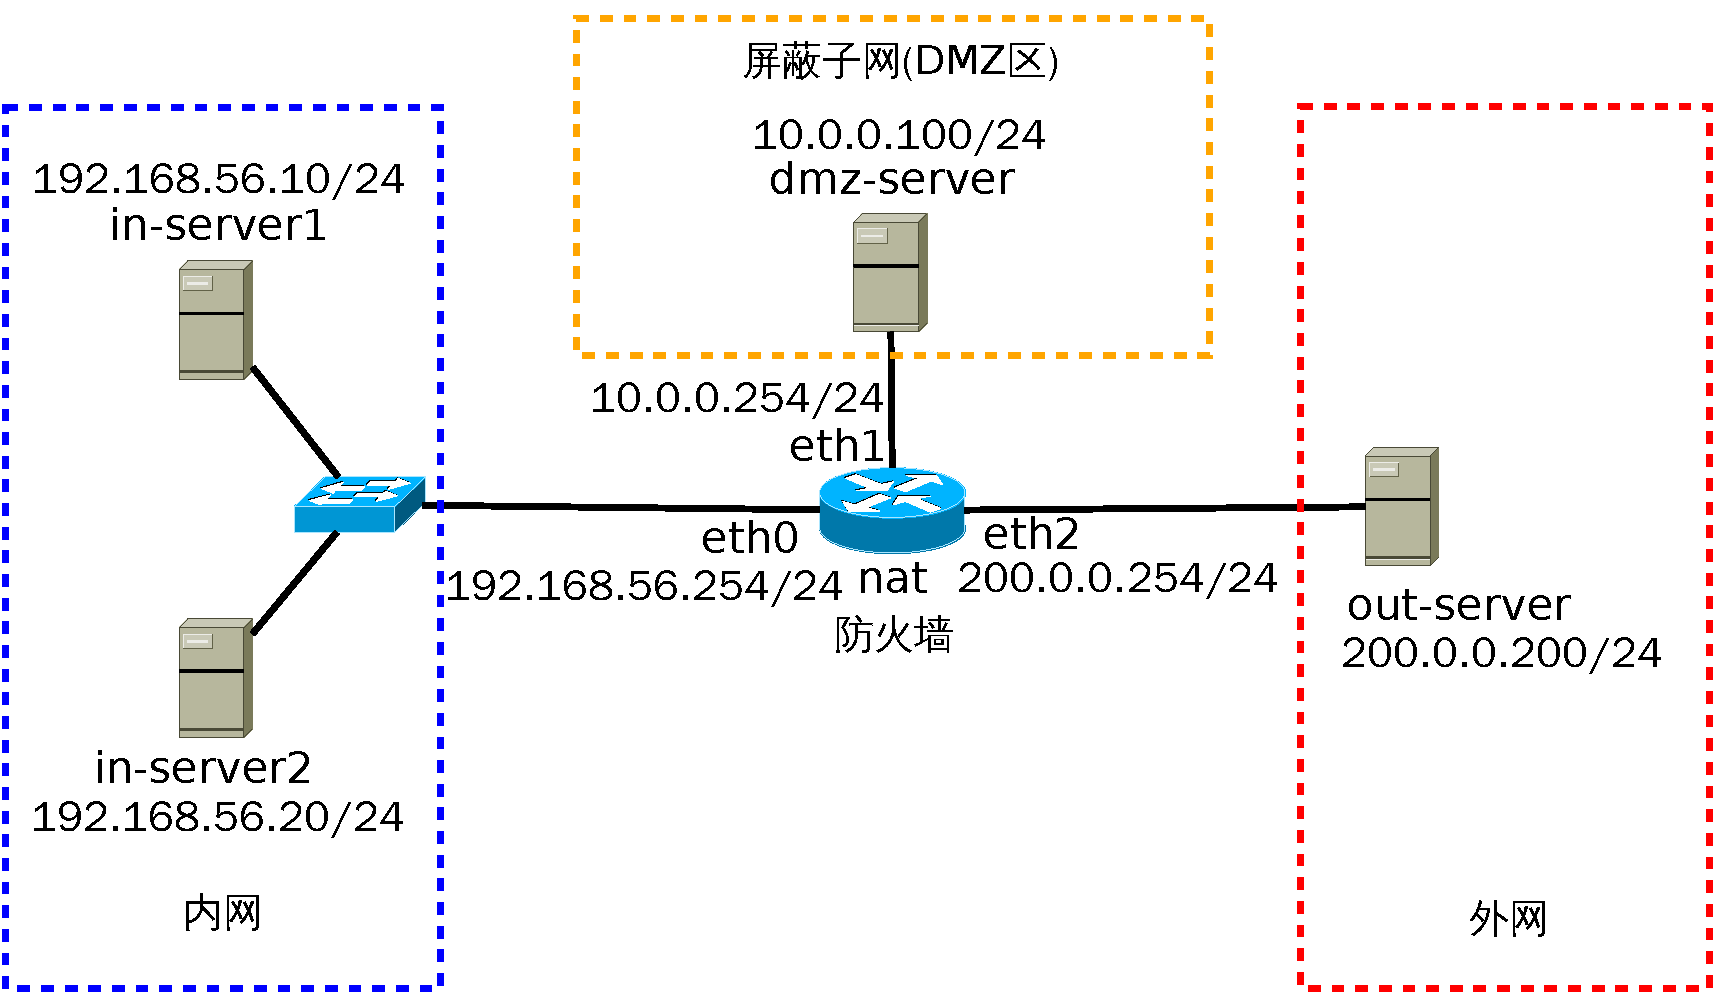
\includegraphics[width=.9\linewidth]{img/dmzlab.pdf}
\end{frame}
\begin{frame}
\frametitle{案例需求}
\label{sec-5-2}
\begin{itemize}

\item 内网、外网
\label{sec-5-2-1}%
\begin{itemize}

\item 搭建web服务器
\label{sec-5-2-1-1}%

\item 配置dns客户端
\label{sec-5-2-1-2}%
\end{itemize} % ends low level

\item dmz区
\label{sec-5-2-2}%
\begin{itemize}

\item 为内外网客户提供dns服务(利用视图)
\label{sec-5-2-2-1}%
\begin{itemize}

\item 内网:abc.com
\label{sec-5-2-2-1-1}%

\item 外网:xyz.net
\label{sec-5-2-2-1-2}%
\end{itemize} % ends low level

\item 提供ftp服务
\label{sec-5-2-2-2}%

\item 为内网客户提供http透明代理上网服务
\label{sec-5-2-2-3}%

\item 为内网服务器提供http反向代理服务
\label{sec-5-2-2-4}%
\end{itemize} % ends low level

\item 防火墙
\label{sec-5-2-3}%
\begin{itemize}

\item 提供数据包过滤服务
\label{sec-5-2-3-1}%

\item 提供内网访问外网服务器的SNAT功能
\label{sec-5-2-3-2}%

\item 提供外网访问内网服务器的DNAT功能
\label{sec-5-2-3-3}%

\item 提供内网透明代理的http劫持功能
\label{sec-5-2-3-4}%
\end{itemize} % ends low level
\end{itemize} % ends low level
\end{frame}
\begin{frame}[fragile]
\frametitle{案例实施(1)}
\label{sec-5-3}
\begin{itemize}

\item 1. 配置主机名、IP地址等,确保网络通畅
\label{sec-5-3-1}%
\begin{itemize}

\item 注意,为了让内网主机和dmz区主机分别通过NAT转换为外部IP地址,需要为防火墙的外网接口再增加一个IP地址,可配置eth2:0子接口ip地址为200.0.0.253\\
\label{sec-5-3-1-1}%
\begin{minted}[]{bash}
cd /etc/sysconfig/network-scripts
vim ifcfg-eth2:0
DEVICE=eth2:0
BOOTPROTO=none
IPADDR=200.0.0.253
NETMASK=255.255.255.0
ONBOOT=yes
\end{minted}

\item 内网源地址通过NAT转换为200.0.0.254
\label{sec-5-3-1-2}%

\item DMZ区源地址通过NAT转换为200.0.0.253
\label{sec-5-3-1-3}%
\end{itemize} % ends low level
\end{itemize} % ends low level
\end{frame}
\begin{frame}[fragile]
\frametitle{案例实施(2)}
\label{sec-5-4}
\begin{itemize}

\item 2. 在dmz-server服务器上配置DNS服务(1)\\
\label{sec-5-4-1}%
\begin{minted}[]{bash}
vim /var/named/chroot/etc/named.conf
options {
        listen-on port 53 { any; };
        directory       "/var/named";
        allow-query     { any; };
        allow-query-cache { any; };
};
#定义内网用户访问控制列表
acl "inside_hosts" {
        127.0.0.1;192.168.56.0/24;10.0.0.0/24;
};
\end{minted}
\end{itemize} % ends low level
\end{frame}
\begin{frame}[fragile]
\frametitle{案例实施(3)}
\label{sec-5-5}
\begin{itemize}

\item 3. 在dmz-server服务器上配置DNS服务(2)\\
\label{sec-5-5-1}%
\begin{minted}[]{bash}
#定义内网用户视图
view inside {
        match-clients      { inside_hosts };
        match-destinations { any; };
        recursion yes;
        include "/etc/named.rfc1912.zones";
        zone "abc.com" IN {
                type master;
                file "abc.com.zone.in";
        };
        zone "xyz.net" IN {
                type master;
                file "xyz.net.zone";
        };
};
\end{minted}
\end{itemize} % ends low level
\end{frame}
\begin{frame}[fragile]
\frametitle{案例实施(4)}
\label{sec-5-6}
\begin{itemize}

\item 3. 在dmz-server服务器上配置DNS服务(3)\\
\label{sec-5-6-1}%
\begin{minted}[]{bash}
#定义其他用户的视图
view outside {
        match-clients  { any; };
        match-destinations { any; };
        recursion no;
        include "/etc/named.rfc1912.zones";
        zone "abc.com" IN {
                type master;
                file "abc.com.zone.out";
        };
        zone "xyz.net" IN {
                type master;
                file "xyz.net.zone";
        };
};
\end{minted}
\end{itemize} % ends low level
\end{frame}
\begin{frame}[fragile]
\frametitle{案例实施(5)}
\label{sec-5-7}
\begin{itemize}

\item 3. 在dmz-server服务器上配置DNS服务(4)\\
\label{sec-5-7-1}%
\begin{minted}[]{bash}
cd /var/named/chroot/var/named
vim abc.com.zone.in
$TTL 86400
@       IN SOA ns1 root (
                        42      ; serial (d. adams)
                        3H      ; refresh
                        15M     ; retry
                        1W      ; expiry
                        1D )    ; minimum
        IN NS           ns1
ns1     IN A            10.0.0.100
www     IN A            192.168.56.10
        IN A            192.168.56.20
ftp     IN CNAME        www
\end{minted}
\end{itemize} % ends low level
\end{frame}
\begin{frame}[fragile]
\frametitle{案例实施(6)}
\label{sec-5-8}
\begin{itemize}

\item 3. 在dmz-server服务器上配置DNS服务(5)\\
\label{sec-5-8-1}%
\begin{minted}[]{bash}
vim abc.com.zone.out
$TTL 86400
@       IN SOA ns1 root (
                        42      ; serial (d. adams)
                        3H      ; refresh
                        15M     ; retry
                        1W      ; expiry
                        1D )    ; minimum
        IN NS           ns1
ns1     IN A            200.0.0.253
www     IN A            200.0.0.253
ftp     IN CNAME        www
\end{minted}
\end{itemize} % ends low level
\end{frame}
\begin{frame}[fragile]
\frametitle{案例实施(7)}
\label{sec-5-9}
\begin{itemize}

\item 3. 在dmz-server服务器上配置DNS服务(6)\\
\label{sec-5-9-1}%
\begin{minted}[]{bash}
vim xyz.net.zone
$TTL 86400
@       IN SOA ns1 root (
                        42      ; serial (d. adams)
                        3H      ; refresh
                        15M     ; retry
                        1W      ; expiry
                        1D )    ; minimum
        IN NS           ns1
ns1     IN A            10.0.0.100
www     IN A            200.0.0.200
ftp     IN CNAME        www

chkconfig --level 345 named on; service named start
\end{minted}
\end{itemize} % ends low level
\end{frame}
\begin{frame}[fragile]
\frametitle{案例实施(8)}
\label{sec-5-10}
\begin{itemize}

\item 4. 配置dns客户端
\label{sec-5-10-1}%
\begin{itemize}

\item 内网和DMZ区客户端\\
\label{sec-5-10-1-1}%
\begin{minted}[]{bash}
vim /etc/resolv.conf
nameserver 10.0.0.100
search localdomain
\end{minted}

\item 外网客户端\\
\label{sec-5-10-1-2}%
\begin{minted}[]{bash}
vim /etc/resolv.conf
nameserver 200.0.0.253
search localdomain
\end{minted}

\item 测试:内网和DMZ区客户端可以解析域名,外网客户端暂时无法解析域名。
\label{sec-5-10-1-3}%
\end{itemize} % ends low level
\end{itemize} % ends low level
\end{frame}
\begin{frame}[fragile]
\frametitle{案例实施(9)}
\label{sec-5-11}
\begin{itemize}

\item 5. 配置防火墙,使外网客户端可以访问DMZ区服务器\\
\label{sec-5-11-1}%
\begin{minted}[]{bash}
vim firewall.sh
iptables -F; iptables -Z
iptables -t nat -F; iptables -t nat -Z
#对http服务的访问转向DMZ区反向代理
iptables -t nat -A PREROUTING -i eth2 -p tcp \
--dport 80 -j DNAT --to 10.0.0.100:80
#对ftp服务的访问转向DMZ区ftp服务器
iptables -t nat -A PREROUTING -i eth2 -p tcp \
--dport 21 -j DNAT --to 10.0.0.100:21
#对dns服务的访问转向DMZ区dns服务器
iptables -t nat -A PREROUTING -i eth2 -p udp \
--dport 53 -j DNAT --to 10.0.0.100:53
service iptables save
\end{minted}
\end{itemize} % ends low level
\end{frame}
\begin{frame}
\frametitle{案例实施(10)}
\label{sec-5-12}
\begin{itemize}

\item 6. 阶段测试
\label{sec-5-12-1}%
\begin{itemize}

\item 外网客户端再次测试dns服务
\label{sec-5-12-1-1}%

\item 外网服务器安装启动http服务
\label{sec-5-12-1-2}%

\item dmz区服务器安装启动ftp服务
\label{sec-5-12-1-3}%

\item 内网服务器安装启动http服务(设置基于IP的虚拟主机)
\label{sec-5-12-1-4}%

\item 测试内、外网访问ftp服务
\label{sec-5-12-1-5}%

\item 测试内访问外网http服务
\label{sec-5-12-1-6}%

\item 测试外网访问内网http服务
\label{sec-5-12-1-7}%
\end{itemize} % ends low level
\end{itemize} % ends low level
\end{frame}
\begin{frame}[fragile]
\frametitle{案例实施(11)}
\label{sec-5-13}
\begin{itemize}

\item 7. 配置DMZ区服务器对内网http服务的反向代理(1)
\label{sec-5-13-1}%
\begin{itemize}

\item 配置squid服务器\\
\label{sec-5-13-1-1}%
\begin{minted}[]{bash}
cd /etc/squid/
cp -p squid.conf squid.conf.bak
sed -i '/^#\|^$/d' squid.conf #去除注释行和空行
vim squid.conf  #在最前面添加(反向代理必须设在最前面)
visible_hostname 10.0.0.100
http_port 80 vhost
cache_peer 192.168.56.10 parent 80 0 \
no-query originserver name=a
cache_peer_domain a www.abc.com
acl all src 0.0.0.0/0.0.0.0
http_access allow all
cache_peer_access a allow all
\end{minted}
\end{itemize} % ends low level
\end{itemize} % ends low level
\end{frame}
\begin{frame}[fragile]
\frametitle{案例实施(12)}
\label{sec-5-14}
\begin{itemize}

\item 7. 配置DMZ区服务器对内网http服务的反向代理(2)
\label{sec-5-14-1}%
\begin{itemize}

\item 启动squid服务器\\
\label{sec-5-14-1-1}%
\begin{minted}[]{bash}
squid -k parse #检查配置文件是否正确
squid -z       #初始化squid缓存
service squid start #启动squid
\end{minted}

\item 外网再次测试访问内外http服务器
\label{sec-5-14-1-2}%
\end{itemize} % ends low level
\end{itemize} % ends low level
\end{frame}
\begin{frame}[fragile]
\frametitle{案例实施(13)}
\label{sec-5-15}
\begin{itemize}

\item 8. 配置DMZ区服务器为内网客户端的http透明代理(1)
\label{sec-5-15-1}%
\begin{itemize}

\item 配置防火墙将内网http数据包重定向至透明代理\\
\label{sec-5-15-1-1}%
\begin{minted}[]{bash}
iptables -t nat -A PREROUTING -i eth0 -p tcp \
--dport 80 -j DNAT --to 10.0.0.100:3128
service iptables save
\end{minted}

\item 测试内网访问外网
\label{sec-5-15-1-2}%
\end{itemize} % ends low level
\end{itemize} % ends low level
\end{frame}
\begin{frame}[fragile]
\frametitle{案例实施(14)}
\label{sec-5-16}
\begin{itemize}

\item 8. 配置DMZ区服务器的http透明代理(2)
\label{sec-5-16-1}%
\begin{itemize}

\item 配置squid服务器\\
\label{sec-5-16-1-1}%
\begin{minted}[]{bash}
vim /etc/squid/squid.conf #在反向代理的配置后面添加
http_port 10.0.0.100:3128 transparent #透明代理
dns_nameservers 127.0.0.1 #指定代理的dns服务器
acl inside src 192.168.56.0/255.255.255.0 #定义内网列表
http_access allow inside #允许内网访问透明代理
\end{minted}

\item 重启squid服务器\\
\label{sec-5-16-1-2}%
\begin{minted}[]{bash}
service squid restart
\end{minted}

\item 再次测试内网访问外网
\label{sec-5-16-1-3}%
\end{itemize} % ends low level
\end{itemize} % ends low level
\end{frame}
\begin{frame}
\frametitle{案例实施(15)}
\label{sec-5-17}
\begin{itemize}

\item 9. 通过防火墙对各种数据包进行限制
\label{sec-5-17-1}%
\begin{itemize}

\item 可以根据具体的安全需求进一步加强防火墙的设置
\label{sec-5-17-1-1}%
\end{itemize} % ends low level
\end{itemize} % ends low level
\end{frame}

\end{document}
